\documentclass[12pt,a4paper,oneside]{report}

% ---------------------------------------------------------------- packages
\usepackage[a4paper,left=1.15in,right=0.95in,top=0.9in,bottom=0.9in]{geometry}
\usepackage[T1]{fontenc}
\usepackage{newtxtext,newtxmath}
\usepackage{setspace}
\usepackage{graphicx}
\usepackage{booktabs,tabularx,multirow,array}
\usepackage{amsmath,bm}
\usepackage[labelsep=colon,font=small,labelfont=bf]{caption}
\usepackage{float}
\usepackage{titlesec}
\usepackage[titles]{tocloft}
\usepackage{enumitem}
\usepackage{xcolor}
\usepackage[numbers,sort&compress]{natbib}
\usepackage{xurl}
\usepackage[hidelinks]{hyperref}

\graphicspath{{figures/}}
\setstretch{1.1}
\setlength{\parskip}{3pt}
\setlength{\emergencystretch}{2.5em}
\setlist{itemsep=2pt,topsep=4pt}
\setlength{\textfloatsep}{16pt plus 4pt minus 2pt}
\setlength{\floatsep}{14pt plus 4pt minus 2pt}
\setlength{\intextsep}{14pt plus 4pt minus 2pt}
\setlength{\abovecaptionskip}{8pt}
\renewcommand{\topfraction}{0.85}
\renewcommand{\textfraction}{0.12}
\renewcommand{\floatpagefraction}{0.75}

% ---------------------------------------------------------------- report details (edit here)
\newcommand{\ReportTitle}{Reinforcement Learning for Swarm Technologies of Drone}
\newcommand{\Supervisor}{Prof.\ Jyotsna Singh}
\newcommand{\SupervisorDesignation}{Professor}
\newcommand{\Department}{Department of Electronics and Communication Engineering}
\newcommand{\Programme}{B.Tech.\ in Electronics \& Communication Engineering}
\newcommand{\University}{Netaji Subhas University of Technology}
\newcommand{\SubmissionMonth}{September 2026}

% ---------------------------------------------------------------- chapter style as in the NSUT demo report
\titleformat{\chapter}[display]{\normalfont\bfseries\centering}{\Large CHAPTER \thechapter}{6pt}{\LARGE\MakeUppercase}
\titlespacing*{\chapter}{0pt}{-12pt}{16pt}
\titleformat{\section}{\normalfont\large\bfseries}{\thesection}{0.8em}{}
\titleformat{\subsection}{\normalfont\normalsize\bfseries}{\thesubsection}{0.8em}{}
\titlespacing*{\section}{0pt}{14pt}{6pt}
\titlespacing*{\subsection}{0pt}{10pt}{4pt}
\renewcommand{\cftchapfont}{\bfseries}
\renewcommand{\cftchappagefont}{\bfseries}
\renewcommand{\cftchapleader}{\cftdotfill{\cftdotsep}}
\setlength{\cftbeforechapskip}{1pt}
\setlength{\cftbeforesecskip}{0pt}
\setlength{\bibsep}{3pt}
\renewcommand{\bibname}{Bibliography}
\numberwithin{equation}{chapter}
\setcounter{tocdepth}{1}

% Version switch: define \WithoutLists before this file (see main_without_lists.tex) to omit the lists of
% figures and tables and their entries in the table of contents.
\newif\ifwithlists
\ifdefined\WithoutLists \withlistsfalse \else \withliststrue \fi

\begin{document}

% ================================================================ TITLE PAGE
\begin{titlepage}
\newgeometry{left=1in,right=1in,top=0.9in,bottom=0.9in}
\centering
\setstretch{1.15}
{\Large\bfseries B.TECH.\ PROJECT ON\par}
\vspace{0.7cm}
{\huge\bfseries Reinforcement Learning for Swarm\\[4pt] Technologies of Drone\par}
\vspace{1.0cm}
{\large\itshape Submitted By\par}
\vspace{0.3cm}
{\large
\begin{tabular}{l@{\hspace{1.2cm}}l}
Nishant Raj    & 2023UEC2606\\
Sumit Kumar    & 2023UEC2554\\
Dheeraj Sharma & 2023UEC2599\\
Tarun Kumar    & 2023UEC2551\\
\end{tabular}\par}
\vspace{0.9cm}
{\large\itshape Under the Guidance of\par}
\vspace{0.25cm}
{\Large\bfseries \Supervisor\par}
{\normalsize \SupervisorDesignation, \Department\par}
\vfill

\includegraphics[width=0.19\textwidth]{nsut_logo}\par
\vfill
{\normalsize Project-I in partial fulfillment of requirement for the award of\par}
{\large\bfseries \Programme\par}
\vspace{0.8cm}
{\large\bfseries \Department\par}
{\large\bfseries NETAJI SUBHAS UNIVERSITY OF TECHNOLOGY\par}
{\large\bfseries NEW DELHI -- 110078\par}
\vspace{0.5cm}
{\large \SubmissionMonth\par}
\restoregeometry
\end{titlepage}

\pagenumbering{roman}
\setcounter{page}{1}

% ================================================================ CERTIFICATE
\chapter*{CERTIFICATE}
\addcontentsline{toc}{chapter}{Certificate}
\begingroup
\setstretch{1.6}
\setlength{\parskip}{12pt}
\sloppy
\vspace*{0.6cm}

Certified that \textbf{Nishant Raj (2023UEC2606)}, \textbf{Sumit Kumar (2023UEC2554)}, \textbf{Dheeraj Sharma
(2023UEC2599)} and \textbf{Tarun Kumar (2023UEC2551)} have carried out their project work presented in this
project entitled \textbf{``\ReportTitle''} for the award of Bachelor of Technology, \Department, \University,
New Delhi, under my supervision.

The project embodies results of original work, and studies are carried out by the students themselves, and the
contents of the project do not form the basis for the award of any other degree to the candidates or to anybody
else from this or any other University/Institution.

\vfill
\noindent
\begin{minipage}[b]{0.45\textwidth}
Place: New Delhi\\[10pt]
Date: \rule{3.5cm}{0.4pt}
\end{minipage}\hfill
\begin{minipage}[b]{0.48\textwidth}
\centering
\rule{5.5cm}{0.4pt}\\[4pt]
\textbf{\Supervisor}\\
\SupervisorDesignation\\
\Department\\
\University, New Delhi
\end{minipage}
\vspace*{1.2cm}
\endgroup

% ================================================================ DECLARATION
\chapter*{CANDIDATES' DECLARATION}
\addcontentsline{toc}{chapter}{Candidates' Declaration}
\begingroup
\setstretch{1.6}
\setlength{\parskip}{12pt}
\vspace*{0.6cm}

We hereby declare that the work presented in this project report entitled \textbf{``\ReportTitle''}, submitted
in partial fulfillment of the requirement for the award of the degree of Bachelor of Technology in Electronics
and Communication Engineering, \University, New Delhi, is an authentic record of our own work carried out under
the guidance of \textbf{\Supervisor}.

The matter embodied in this report has not been submitted by us for the award of any other degree. Wherever the
work of others has been used, it has been duly acknowledged and cited.

\vfill
\noindent
\begin{tabular*}{\textwidth}{@{\extracolsep{\fill}}cc}
\rule{5cm}{0.4pt} & \rule{5cm}{0.4pt}\\
\textbf{Nishant Raj} & \textbf{Sumit Kumar}\\
2023UEC2606 & 2023UEC2554\\[1.6cm]
\rule{5cm}{0.4pt} & \rule{5cm}{0.4pt}\\
\textbf{Dheeraj Sharma} & \textbf{Tarun Kumar}\\
2023UEC2599 & 2023UEC2551\\
\end{tabular*}

\vspace{1cm}
\noindent Place: New Delhi \hfill Date: \rule{3.5cm}{0.4pt}
\vspace*{1.2cm}
\endgroup

% ================================================================ ACKNOWLEDGEMENT
\chapter*{ACKNOWLEDGEMENT}
\addcontentsline{toc}{chapter}{Acknowledgement}
\begingroup
\setstretch{1.6}
\setlength{\parskip}{12pt}
\vspace*{0.6cm}

We would like to express our gratitude and appreciation to all those who made it possible to complete this
project.

Special thanks to our project supervisor, \textbf{\Supervisor}, whose guidance, stimulating suggestions and
encouragement helped us throughout the design, implementation and evaluation of this work.

We also sincerely thank the \Department, \University, for providing the facilities and environment required
for the project, and our colleagues for their valuable support and assistance throughout the project.

\vfill
\noindent
\begin{tabular*}{\textwidth}{@{\extracolsep{\fill}}cc}
\rule{5cm}{0.4pt} & \rule{5cm}{0.4pt}\\
\textbf{Nishant Raj} & \textbf{Sumit Kumar}\\[1.6cm]
\rule{5cm}{0.4pt} & \rule{5cm}{0.4pt}\\
\textbf{Dheeraj Sharma} & \textbf{Tarun Kumar}\\
\end{tabular*}
\vspace*{1.2cm}
\endgroup

% ================================================================ ABSTRACT
\chapter*{ABSTRACT}
\addcontentsline{toc}{chapter}{Abstract}
This work presents a reinforcement-learning system for the cooperative control of a drone swarm. Eight drones
follow a moving reference target in a fixed formation; when a non-cooperative object crosses the flight path,
the drones leave their formation slots, avoid the object and one another, and then return to \emph{their own}
slots relative to the moving target. A single neural policy is shared by all drones and each drone executes it
using only local observations of its own state, its six nearest neighbours and up to six nearby objects. The
policy combines a self encoder with attention-based set encoders, so that it is independent of the order in
which neighbours are observed, and outputs a desired three-dimensional velocity to a stabilised flight model.

The environment is implemented as a PettingZoo multi-agent environment with continuous swept collision
detection, a bounded per-drone reward and an explicit formation-recovery criterion. Training uses a three-stage
curriculum: in each stage the policy is first initialised from demonstrations of a sampling-based
model-predictive expert planner (noise-injected demonstrations followed by DAgger) and is then fine-tuned with
proximal policy optimisation (PPO) and generalised advantage estimation, while the best checkpoint is selected on
separate validation seeds.

The final model was evaluated on 140 held-out episodes (seven scenarios $\times$ 20 unseen seeds). It completed
138 episodes (98.6\%) without failure, achieved 100\% success in six of the seven scenarios, kept the
undisturbed formation error below 5\,cm (0.023--0.045\,m) and returned every drone to its own slot after every
disturbance in the completed episodes. A browser-based flight laboratory visualises the learned behaviour
interactively.

\vspace{0.5cm}
\noindent\textbf{Keywords:} multi-agent reinforcement learning, drone swarm, formation control, collision
avoidance, proximal policy optimisation, attention, imitation learning.

% ================================================================ LISTS (each on its own page)
\clearpage
{\small\setstretch{0.97}\tableofcontents}
\ifwithlists
\clearpage
\phantomsection
\addcontentsline{toc}{chapter}{List of Figures}
{\setstretch{1.1}\listoffigures}
\clearpage
\phantomsection
\addcontentsline{toc}{chapter}{List of Tables}
{\setstretch{1.1}\listoftables}
\fi


\clearpage
\pagenumbering{arabic}
\chapter{Introduction}
\label{ch:introduction}

\section{General}
A drone swarm is a group of unmanned aerial vehicles that cooperate to perform a task that a single vehicle
cannot perform as efficiently, such as area coverage, inspection, search and rescue, or aerial display.
Instead of being flown individually, the drones must coordinate their motion: they have to keep a desired
geometric arrangement, avoid colliding with one another, and react to objects in the environment. Classical
approaches describe such behaviour with hand-designed rules and geometric collision-avoidance methods
\cite{vandenberg2011reciprocal}.

Deep reinforcement learning (RL) offers an alternative in which the control law is \emph{learned} from
interaction with a simulator. RL has produced decentralised controllers for quadrotor swarms that keep
formations and avoid obstacles \cite{batra2021decentralized,huang2024collision}. In this multi-agent setting,
every drone is an agent that observes only its local surroundings, and the swarm-level behaviour emerges from
many agents executing the same learned policy \cite{yu2022surprising}.

This project, titled \emph{Reinforcement Learning for Swarm Technologies of Drone}, develops such a system.
The implemented software, named \textbf{SwarmFlow}, trains one shared neural policy that lets a swarm of eight
drones follow a moving reference target, yield to crossing objects and recover its formation.
Figure~\ref{fig:overview} summarises the complete system.

\begin{figure}[htbp]
  \centering
  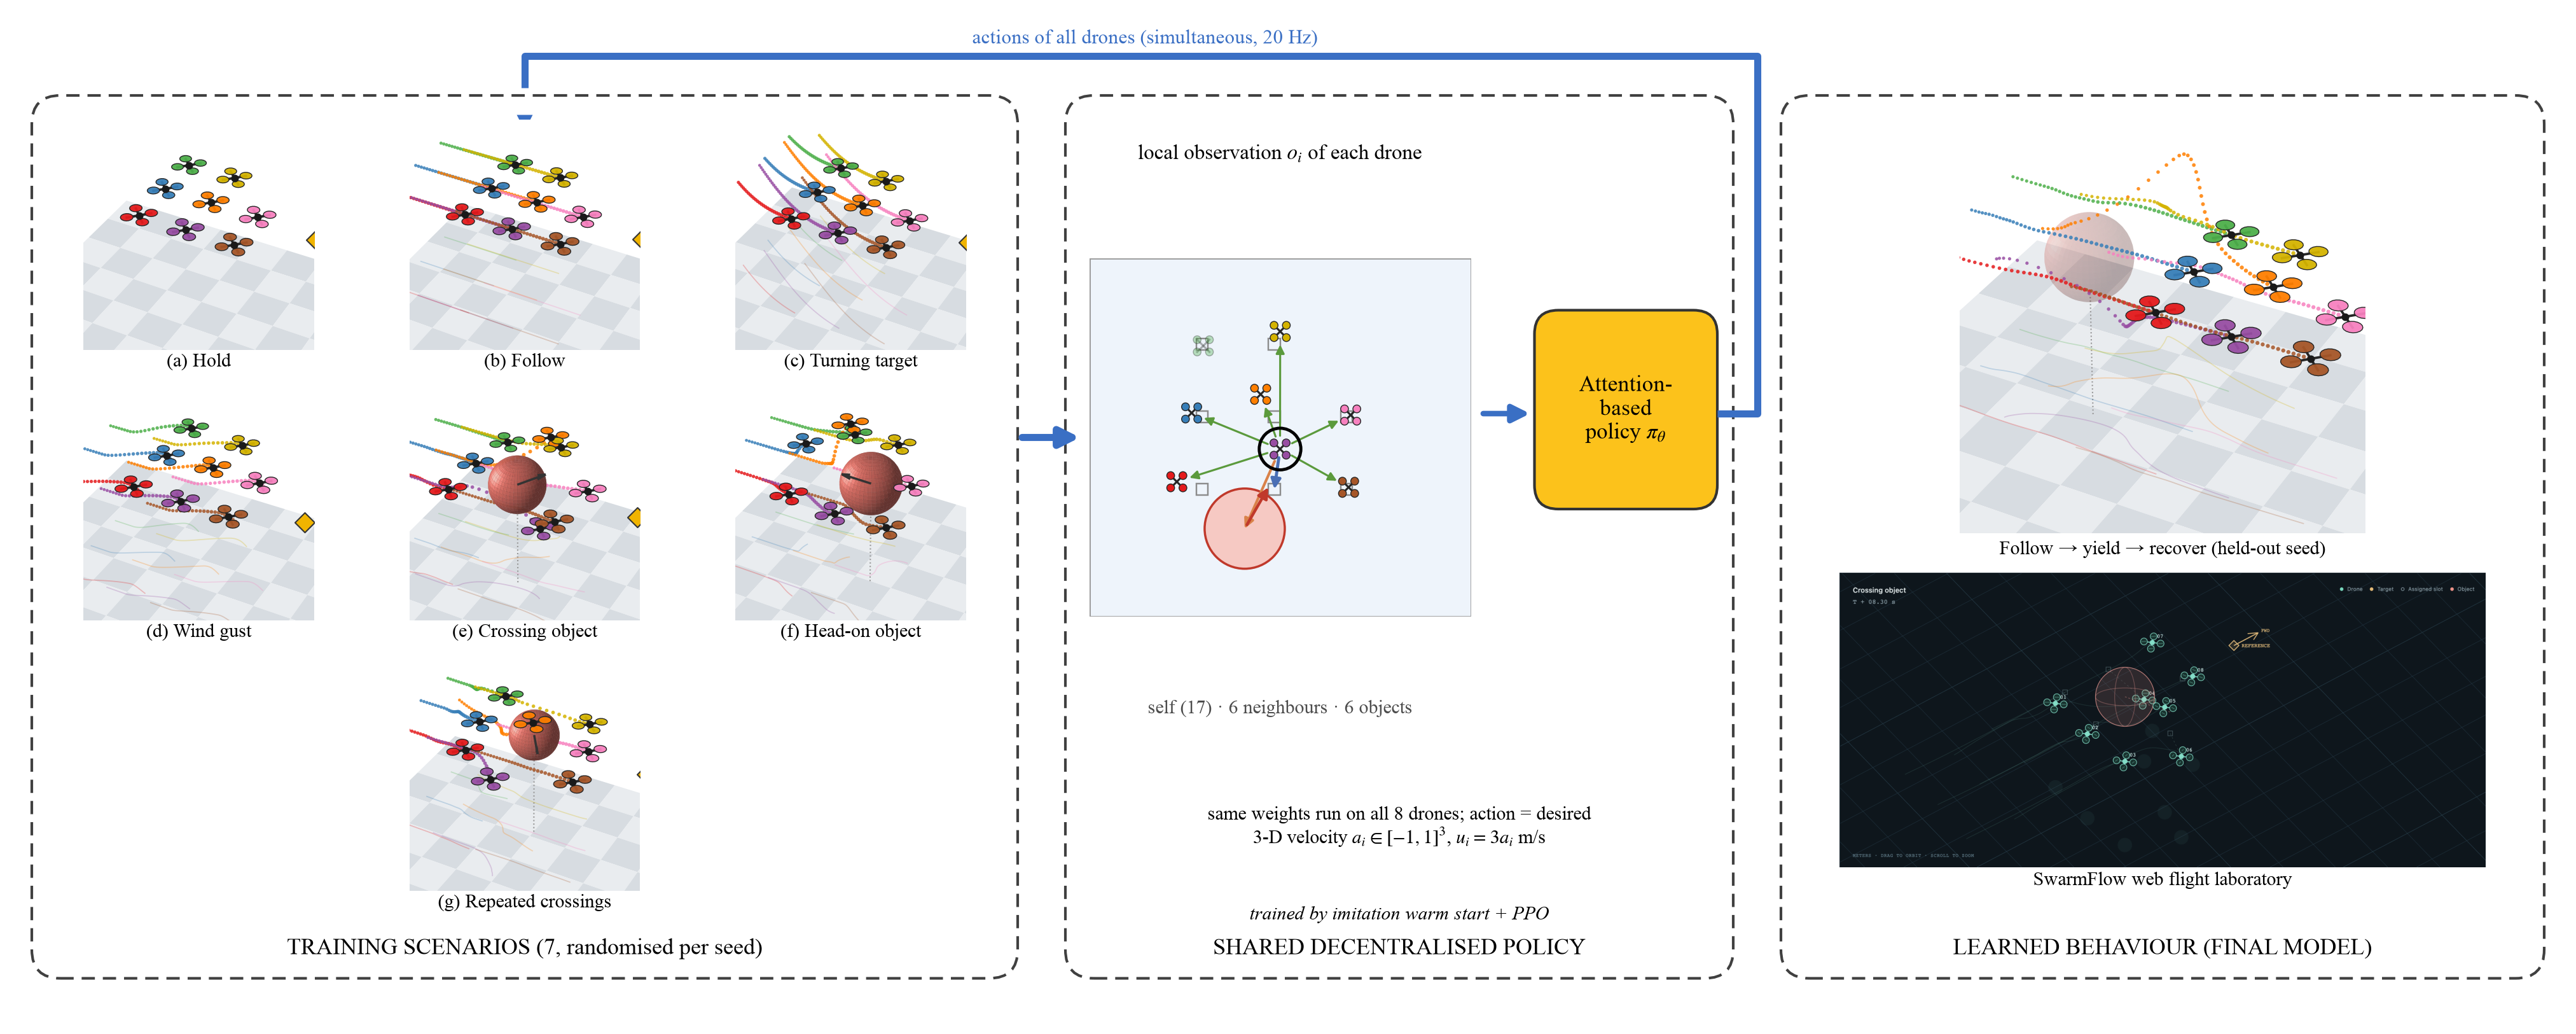
\includegraphics[width=0.84\textwidth]{fig_system_overview}
  \caption[Overview of the proposed reinforcement-learning drone-swarm system]{Overview of the proposed system.
  Left: the seven training scenarios, rendered from the simulator. Middle: every drone builds a local
  observation and the shared attention-based policy maps it to a velocity command; the actions of all drones
  are applied simultaneously. Right: behaviour of the final model on a held-out seed and the web-based flight
  laboratory.}
  \label{fig:overview}
\end{figure}

\section{Need for the Study}
Formation flight with obstacle avoidance involves several requirements that conflict with each other. A drone
that stays exactly in its slot may collide with an approaching object; a drone that avoids the object must
not collide with its neighbours; and after the disturbance the formation must be restored, with every drone
returning to its own place rather than to any free position. Encoding all of these interactions by hand
becomes difficult as the number of drones and the variety of disturbances increase.

A learned, decentralised controller is attractive because the same policy runs on every drone, it uses only
locally available information, and it can in principle be applied to different swarm sizes. However, training
such a controller from scratch is sample-inefficient: published quadrotor-swarm results use very large
training budgets \cite{batra2021decentralized}. A practical project therefore needs a formulation that learns
swarm coordination efficiently on ordinary computing hardware while remaining measurable and reproducible.

\section{Problem Statement}
\label{sec:problem}
The problem considered in this work is to learn a single decentralised policy $\pi_\theta$ for a swarm of
$N=8$ drones such that:
\begin{enumerate}
  \item every drone follows its own persistent formation slot, defined 3\,m behind a reference target that
        moves along a prescribed path;
  \item when a spherical object crosses the formation (laterally, head-on, or repeatedly), the drones avoid
        the object and each other without any collision;
  \item after the object leaves, every drone returns to \emph{its own} slot relative to the moving target;
  \item each drone uses only local, relative observations and the policy weights are shared by all drones.
\end{enumerate}
The behaviour is evaluated on scenarios with unseen random seeds using three measurable criteria: absence of
collisions, formation recovery within 5\,s, and a slot root-mean-square error (RMSE) below 0.35\,m when the
formation is undisturbed.

\section{Objectives}
\begin{enumerate}
  \item To build a multi-agent simulation environment for formation following, obstacle yielding and formation
        recovery with continuous collision detection.
  \item To formulate the task as a decentralised multi-agent RL problem with local observations, continuous
        velocity actions and a bounded reward.
  \item To design a permutation-invariant, attention-based policy network shared by all drones.
  \item To train the policy with a curriculum that combines demonstration-guided initialisation and PPO.
  \item To evaluate the final model on held-out seeds and to demonstrate it in an interactive web viewer.
\end{enumerate}

\section{Scope of the Work}
The drones are simulated with a stabilised velocity-level flight model: the policy commands a desired velocity
and a lower-level controller with finite response time and bounded acceleration tracks it. The learning
therefore concentrates on swarm coordination rather than on rotor-level stabilisation, an approach motivated by
the separation of control levels in \cite{panerati2021learning}. Obstacles are modelled as spheres, sensing is
ideal by default, and the reference target follows a scripted path. Full rotor dynamics and hardware flight
are outside the present scope and are discussed as future work in Chapter~\ref{ch:results}.

\chapter{Literature Review}
\label{ch:literature}

This chapter reviews the works on which the design of this project is directly based.

\section{Reinforcement Learning and Policy Optimisation}
In reinforcement learning an agent interacts with an environment, observes states, selects actions and
receives rewards; the objective is a policy that maximises the expected discounted return. For continuous
control, policy-gradient methods optimise a parameterised stochastic policy directly. Proximal Policy
Optimisation (PPO) \cite{schulman2017proximal} restricts each policy update with a clipped probability ratio,
so that the new policy cannot move too far from the policy that collected the data. This makes learning stable
while allowing several optimisation epochs on the same batch of experience. The quality of a policy-gradient
update depends strongly on the estimate of the advantage, i.e.\ how much better an action was than expected.
Generalised Advantage Estimation (GAE) \cite{schulman2016gae} computes this estimate as an exponentially
weighted sum of temporal-difference errors, with a parameter $\lambda$ that trades bias against variance. PPO
with GAE is the optimisation method used in this project.

\section{Multi-Agent Reinforcement Learning for Cooperative Tasks}
When several agents learn together, the environment becomes non-stationary from the point of view of each agent.
Yu et al.\ \cite{yu2022surprising} showed that PPO, often regarded as a single-agent method, is a strong
algorithm for cooperative multi-agent problems when it is combined with parameter sharing among homogeneous
agents and with a small number of implementation choices such as few epochs per batch, a clip parameter of at
most 0.2 and large batches. They compare a local value function (independent PPO) with a centralised value
function (MAPPO) that uses global information during training only. Following this study, our policy is shared
by all drones and trained with PPO and a local critic; the centralised critic is left as an option for future
comparison.

\section{Deep Reinforcement Learning for Quadrotor Swarms}
Batra et al.\ \cite{batra2021decentralized} trained a decentralised policy for quadrotor swarms end-to-end with
PPO (Figure~\ref{fig:lit_batra}). Each drone encodes its own state with a self encoder and the relative positions
and velocities of its neighbours with a permutation-invariant neighbour encoder (deep sets or attention), and the
same policy is shared by all drones. The trained swarms keep and change formations, and in one experiment
re-establish their formation around moving spherical obstacles. The paper also separates collision and formation
measurements, which our evaluation adopts.

\begin{figure}[htbp]
  \centering
  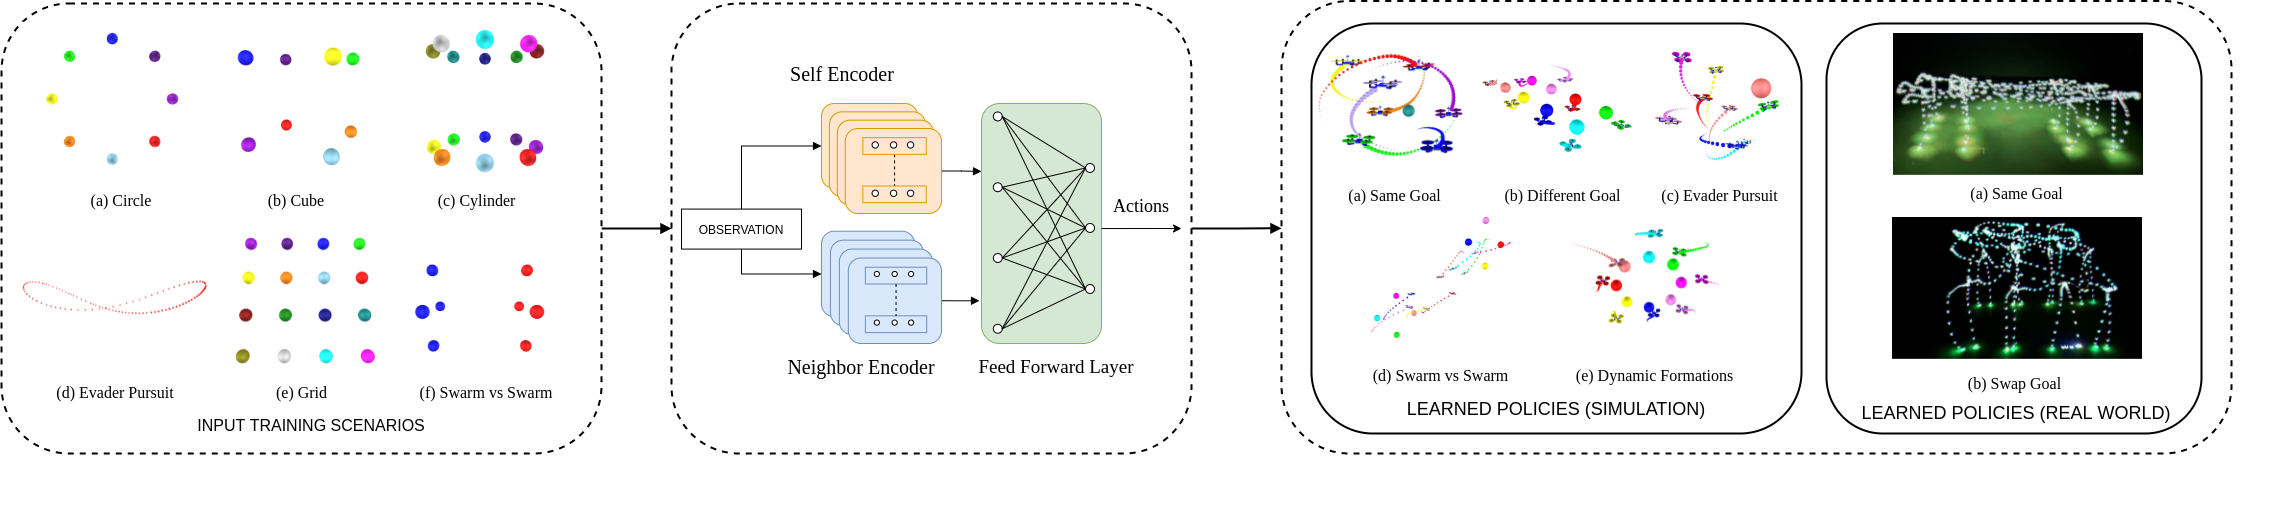
\includegraphics[width=0.7\textwidth]{literature/batra2021_fig1}
  \caption[Decentralised quadrotor-swarm control with shared encoders (Batra et al.)]{Decentralised
  quadrotor-swarm control with self and neighbour encoders trained on randomised formation scenarios.
  Reproduced from Batra et al.\ \cite{batra2021decentralized}.}
  \label{fig:lit_batra}
\end{figure}

Huang et al.\ \cite{huang2024collision} extended this line of work to navigation through obstacle fields. They
add an obstacle encoder, use attention over neighbour and obstacle observations, and introduce a replay mechanism
that restarts training episodes from states shortly before a collision, so that the policy practises difficult
situations more often while still collecting fresh on-policy data. The accompanying QuadSwarm simulator
\cite{huang2023quadswarm} emphasises the separation of the simulation from rendering and a seeded, randomised
generation of scenarios. Our observation structure (self, neighbours, objects), the attention encoders, the
collision-state replay and the separation of the simulator from the web viewer follow these works.

\section{Simulation Environments for Multi-Drone Learning}
Panerati et al.\ \cite{panerati2021learning} introduced gym-pybullet-drones, a multi-agent quadcopter environment
with rigid-body physics and aerodynamic effects, and discussed the choice of the control level at which an RL
agent acts, from motor commands to velocity set-points. This motivates the decision in this project to learn at
the velocity level above a stabilised flight model, which makes training fast enough for ordinary hardware, and
identifies a path for later validation with full quadrotor physics.

\section{Collision Avoidance and Learning from Demonstrations}
Van den Berg et al.\ \cite{vandenberg2011reciprocal} formulated reciprocal collision avoidance for many agents in
terms of the relative positions and velocities of neighbouring agents. Reasoning about relative motion over a
short prediction horizon underlies both the observation design of our policy and the sampling-based expert
planner that provides demonstrations.

Learning from demonstrations reduces the exploration that RL must perform. Plain behaviour cloning suffers from
covariate shift: the learner makes small errors, reaches states that the expert never demonstrated and does not
know how to recover. DAgger \cite{ross2011reduction} removes this problem by letting the learner act, asking the
expert to label every state the learner visits, and training on the aggregated data set. Our pipeline uses DAgger
rounds at the start of every curriculum stage.

\section{Research Gap}
The reviewed swarm-RL works \cite{batra2021decentralized,huang2024collision} learn directly at the thrust level
with very large sample budgets, and their formation tasks do not require a drone to return to its own slot after
an avoidance manoeuvre. Three aspects motivate the present project:
\begin{enumerate}
  \item \textbf{Same-slot recovery as an explicit requirement.} After avoiding an object, each drone must return
        to its own slot relative to a moving target, measured with a quantitative recovery criterion.
  \item \textbf{Training on ordinary hardware.} By learning coordination above a stabilised flight layer
        \cite{panerati2021learning} and initialising each curriculum stage from expert demonstrations
        \cite{ross2011reduction}, the complete training runs on a laptop in a few hours.
  \item \textbf{Held-out, reproducible evaluation.} Training, checkpoint selection and final testing use disjoint
        ranges of random seeds, and every reported number is regenerated from saved files.
\end{enumerate}

\chapter{Mathematical Modelling and Methodology}
\label{ch:method}

This chapter formulates the swarm task as a multi-agent reinforcement-learning problem and describes the
environment model, the observation and action spaces, the reward, the policy network and the learning
algorithm. All constants are the values used by the implementation.

\section{Problem Formulation}
The task is modelled as a decentralised, partially observable Markov game with $N$ identical agents,
\begin{equation}
  \mathcal{G} = \left\langle \mathcal{N}, \mathcal{S}, \{\mathcal{O}_i\}_{i=1}^{N}, \{\mathcal{A}_i\}_{i=1}^{N},
  P, \{r_i\}_{i=1}^{N}, \gamma \right\rangle ,
  \label{eq:game}
\end{equation}
where $\mathcal{S}$ is the full simulator state (positions and velocities of all drones, the target and all
objects), $o_i \in \mathcal{O}_i$ is the local observation of drone $i$, $a_i \in \mathcal{A}_i=[-1,1]^3$ its
action, $P$ the transition model, $r_i$ its reward and $\gamma = 0.99$ the discount factor. All drones execute
the same stochastic policy $\pi_\theta(a_i \mid o_i)$ with shared parameters $\theta$ and act simultaneously
at 20\,Hz. The objective is to maximise the expected discounted return of every drone,
\begin{equation}
  J(\theta) = \mathbb{E}_{\pi_\theta}\Bigl[\sum_{t=0}^{T-1} \gamma^{t}\, r_{i,t}\Bigr],
  \qquad
  V_\phi(o) \approx \mathbb{E}_{\pi_\theta}\Bigl[\sum_{k \ge 0}\gamma^k r_{i,t+k} \Bigm| o_{i,t}=o\Bigr],
  \label{eq:objective}
\end{equation}
where $V_\phi$ is a learned value function (critic) that is used only during training.

\section{Flight Dynamics and Collision Model}
Each drone is a sphere of radius $\rho = 0.18$\,m whose motion is governed by a stabilised velocity-tracking
model. The normalised action is mapped to a desired velocity $u_i = \operatorname{lim}_{3}(3\,a_i)$, where the
operator $\operatorname{lim}_b(x) = x\,\min(1, b/\lVert x\rVert)$ limits the norm of a vector to $b$. Each
50\,ms control step is integrated with five sub-steps of $h = 10$\,ms:
\begin{align}
  \dot v_i &= \operatorname{lim}_{a_{\max}}\!\left(\frac{u_i - v_i}{\tau}\right), \label{eq:dyn1}\\
  v_i &\leftarrow v_i + (\dot v_i + w)\,h, \qquad p_i \leftarrow p_i + v_i\,h, \label{eq:dyn2}
\end{align}
with response time $\tau = 0.28$\,s, acceleration limit $a_{\max} = 5$\,m/s$^2$ and an external disturbance $w$
that is non-zero only in the wind-gust scenario ($w=(0,1.2,0.2)$\,m/s$^2$ for $7 \le t < 9$\,s).

Collisions are detected continuously. For two bodies whose relative position changes linearly from $d_0$ to
$d_1$ during a sub-step, the minimum centre distance is
\begin{equation}
  d_{\min} = \left\lVert d_0 + s^\ast (d_1 - d_0) \right\rVert, \qquad
  s^\ast = \operatorname{clip}\!\left(-\frac{d_0\cdot(d_1-d_0)}{\lVert d_1 - d_0\rVert^2},\,0,\,1\right),
  \label{eq:swept}
\end{equation}
and a collision occurs when the surface gap $d_{\min} - \rho_a - \rho_b \le 0$. This swept test prevents fast
objects from passing through a drone between two samples. A collision, ground contact or leaving the
$\pm 60$\,m, 0--10\,m flight volume ends the episode for the whole team. Table~\ref{tab:env} lists the main
parameters.

\begin{table}[htbp]
\centering
\caption{Simulation parameters of the environment}
\label{tab:env}
\small
\begin{tabular}{@{}llll@{}}
\toprule
Parameter & Value & Parameter & Value\\
\midrule
Drones $N$ & 8 (grid formation) & Control rate / sub-steps & 20\,Hz / 5\\
Drone radius $\rho$ & 0.18\,m & Episode length $T$ & 24\,s (480 steps)\\
Slot spacing & 1.25\,m & Max.\ speed / acceleration & 3\,m/s / 5\,m/s$^2$\\
Stand-off behind target & 3\,m & Response time $\tau$ & 0.28\,s\\
Flight altitude & 3\,m & Target speed & 0.55\,m/s\\
Sensing range & 7\,m & Observed neighbours / objects & 6 / 6\\
\bottomrule
\end{tabular}
\end{table}

\section{Formation and Scenarios}
The reference target moves as $q(t) = (2 + 0.55\,t,\ 0,\ 3)$\,m (it is stationary in the hold scenario and
follows $q_y = 1.8\sin(0.22t)$, $q_z = 3 + 0.35\sin(0.3t)$ in the turning scenario). Drone $i$ owns a
persistent offset $\delta_i$ in a world-aligned grid and its slot is
\begin{equation}
  s_i(t) = q(t) - (3,\,0,\,0) + \delta_i .
  \label{eq:slot}
\end{equation}
The slot assignment never changes within an episode, so recovery means returning to the same $s_i$.
Crossing objects are spheres with radius $r_o$ that start outside the formation and move with constant velocity
$v_o = \dot q(t_0) + v_r\,\hat d$, i.e.\ with relative speed $v_r$ in direction $\hat d$ with respect to the
target. The seven benchmark scenarios are \emph{hold}, \emph{follow}, \emph{turn}, \emph{gust},
\emph{crossing} ($r_o \in [0.6,0.8]$\,m, $v_r \in [1.4,1.8]$\,m/s, lateral), \emph{head-on}
($r_o \in [0.7,0.9]$\,m, $v_r \in [1.8,2.2]$\,m/s, from the front) and \emph{double crossing} (two opposite
crossings 6--10\,s apart). Start times, directions, speeds and radii are randomised by the episode seed.

\section{Observation and Action Spaces}
The observation of drone $i$ contains only local and relative quantities (Figure~\ref{fig:observation}):
\begin{equation}
  o_i = \left( o_i^{\mathrm{self}} \in \mathbb{R}^{17},\;
               O_i^{\mathrm{nbr}} \in \mathbb{R}^{6\times 8},\;
               O_i^{\mathrm{obj}} \in \mathbb{R}^{6\times 8} \right).
  \label{eq:obs}
\end{equation}
Table~\ref{tab:obs} lists the components. Neighbours and objects are sorted by distance, limited to the 7\,m
sensing range and to six rows each; missing rows are zero-padded and masked. No global state, future path or
goal of another drone is observed. The action is the normalised desired velocity $a_i\in[-1,1]^3$.

\begin{figure}[htbp]
  \centering
  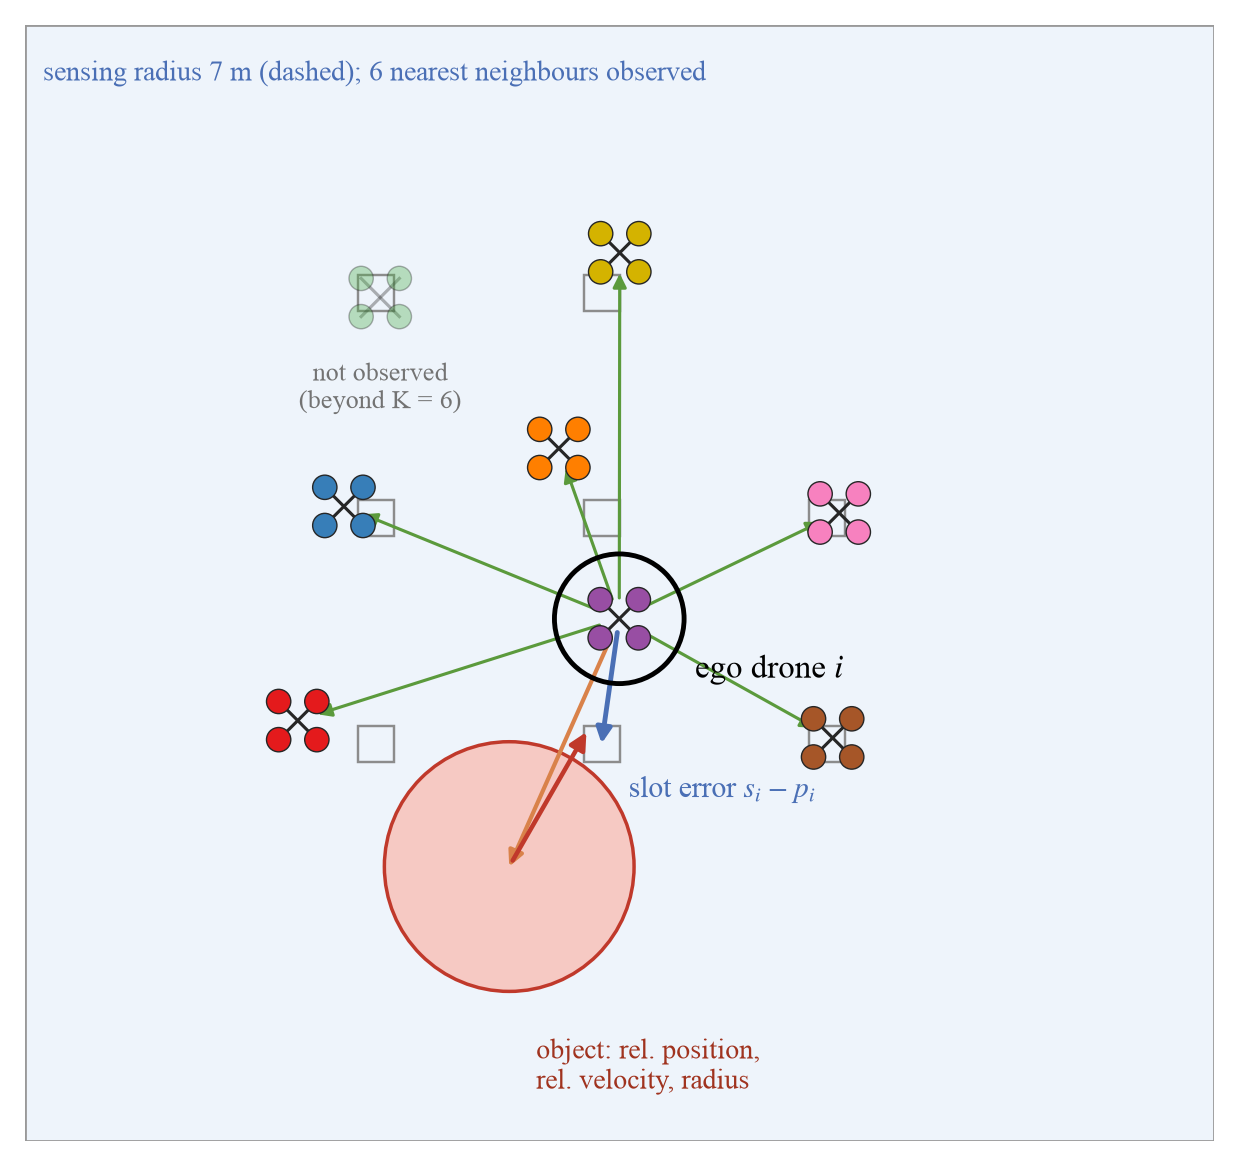
\includegraphics[width=0.48\textwidth]{fig_local_observation}
  \caption[Local observation of one drone]{Local observation of one drone (ego, circled), drawn from a recorded
  simulation state. Green arrows: relative positions of the six nearest neighbours (the seventh drone is not
  observed); orange arrow: relative position of the object, whose velocity is shown in red; blue arrow: slot
  error $s_i - p_i$ to the assigned slot (square).}
  \label{fig:observation}
\end{figure}

\begin{table}[htbp]
\centering
\caption{Observation vector of each drone}
\label{tab:obs}
\small
\begin{tabularx}{\textwidth}{@{}lcX@{}}
\toprule
Part & Size & Content\\
\midrule
$o^{\mathrm{self}}_i$ & 17 & slot error $s_i-p_i$ (3), own velocity (3), target velocity (3), previous command (3),
slot offset $\delta_i$ (3), altitude (1), remaining episode fraction (1)\\
$O^{\mathrm{nbr}}_i$ & $6\times8$ & per neighbour: relative position (3), relative velocity (3), radius (1), validity mask (1)\\
$O^{\mathrm{obj}}_i$ & $6\times8$ & per object: relative position (3), relative velocity (3), radius (1), validity mask (1)\\
\bottomrule
\end{tabularx}
\end{table}

\section{Reward Design}
The reward of drone $i$ at each step is a constant survival term minus a bounded cost,
\begin{equation}
  r_{i,t} = \Delta t\,\bigl(1 - C_{i,t}\bigr) \;-\; 100\cdot\mathbb{1}\!\left[\text{drone } i \text{ involved in a failure}\right],
  \label{eq:reward}
\end{equation}
with $\Delta t = 0.05$\,s. With the slot error $e = \lVert p_i - s_i\rVert$ capped at $e_c = \min(e, 5)$, the
cost is
\begin{equation}
\begin{aligned}
  C ={}& C_{\mathrm{slot}}(e_c) + 0.12\min(\lVert v_i - \dot q\rVert, 3)^2 + 6\,[0.45 - g_{\mathrm{nn}}]_+^2 \\
      &+ 3\min\Bigl(\sum_{o}\bigl[1 - g_o\bigr]_+^2,\, 2\Bigr) + 0.005\lVert u_i\rVert^2
      + 0.001\min\Bigl(\tfrac{\lVert \Delta u_i\rVert}{\Delta t}, 20\Bigr)^2,
\end{aligned}
  \label{eq:cost}
\end{equation}
\begin{equation}
  C_{\mathrm{slot}}(e_c) = \begin{cases} e_c^2, & e_c \le 1\,\text{m},\\ 2e_c - 1, & e_c > 1\,\text{m},\end{cases}
  \label{eq:slotcost}
\end{equation}
where $g_{\mathrm{nn}}$ is the surface gap to the nearest drone, $g_o$ the surface gap (in metres) to each active object
and $[x]_+=\max(0,x)$. Table~\ref{tab:reward} explains each term. Because every cost is capped, the per-step
reward is bounded from below; a unit test confirms that even the worst-case discounted return of a surviving
drone is higher than the $-100$ failure penalty, so ending an episode early is never an easy way to avoid the
costs. The failure penalty is assigned only to the drones involved, so that the learning signal identifies the
responsible agent \cite{batra2021decentralized}.

\begin{table}[htbp]
\centering
\caption{Terms of the per-drone cost}
\label{tab:reward}
\small
\begin{tabularx}{\textwidth}{@{}lcX@{}}
\toprule
Term & Weight & Purpose\\
\midrule
Slot tracking $C_{\mathrm{slot}}$ & 1 & quadratic near the slot, linear far away (bounded gradient)\\
Velocity matching & 0.12 & move with the target velocity\\
Drone proximity & 6 & keep more than 0.45\,m surface gap to the nearest drone\\
Object warning zone & 3 & smooth penalty inside 1\,m of an object, capped at two objects\\
Command effort / rate & 0.005 / 0.001 & smooth, economical velocity commands\\
Failure & $-100$ & collision, ground contact or leaving the flight volume\\
\bottomrule
\end{tabularx}
\end{table}

\section{Policy Network}
The policy (Figure~\ref{fig:network}) follows the self/neighbour/obstacle encoder structure of
\cite{batra2021decentralized,huang2024collision}. The self observation is normalised and encoded by a linear
layer with $\tanh$ activation into $e_{\mathrm{self}}\in\mathbb{R}^{128}$. Each neighbour (or object) row $x_j$ is
encoded by a shared two-layer MLP, $h_j = \phi(x_j)\in\mathbb{R}^{128}$, and the set of rows is pooled by
multi-head attention with a learned query $q$ \cite{huang2024collision}:
\begin{equation}
\begin{aligned}
  \hat e &= \operatorname{MHA}\bigl(q,\,H,\,H\bigr) = \bigl[\operatorname{head}_1,\dots,\operatorname{head}_4\bigr]W^O,\\
  \operatorname{head}_k &= \operatorname{softmax}\Bigl(\frac{qW_k^Q\,(HW_k^K)^\top}{\sqrt{d_k}} + M\Bigr) HW_k^V ,
\end{aligned}
  \label{eq:attention}
\end{equation}
where $H = [h_1,\dots,h_6]$ and the mask $M$ removes padded rows. Because the softmax weights are computed per
row, the result is independent of the order of neighbours \cite{batra2021decentralized}. The three
embeddings are concatenated (384 values) and passed through a trunk MLP (384$\to$256$\to$128). The actor head
outputs the mean $\mu_\theta(o_i)$ of a Gaussian with a learnable, state-independent standard deviation
$\sigma$; the action is squashed with $\tanh$:
\begin{equation}
\begin{aligned}
  &x \sim \mathcal{N}\bigl(\mu_\theta(o_i), \operatorname{diag}\sigma^2\bigr),\qquad a_i = \tanh(x),\\
  &\log\pi_\theta(a_i\mid o_i) = \sum_{k=1}^{3}\Bigl[\log\mathcal{N}(x_k) - \log\bigl(1-\tanh^2 x_k\bigr)\Bigr].
\end{aligned}
  \label{eq:tanh}
\end{equation}
The correction term accounts for the change of variables introduced by the $\tanh$ squashing. At deployment the
deterministic action $a_i = \tanh(\mu_\theta(o_i))$ is used. The critic $V_\phi(o_i)$ has a separate encoder
of the same architecture, so value-loss gradients cannot disturb the actor
features. The actor has 284{,}166 and the critic 283{,}905 trainable parameters.

\begin{figure}[htbp]
  \centering
  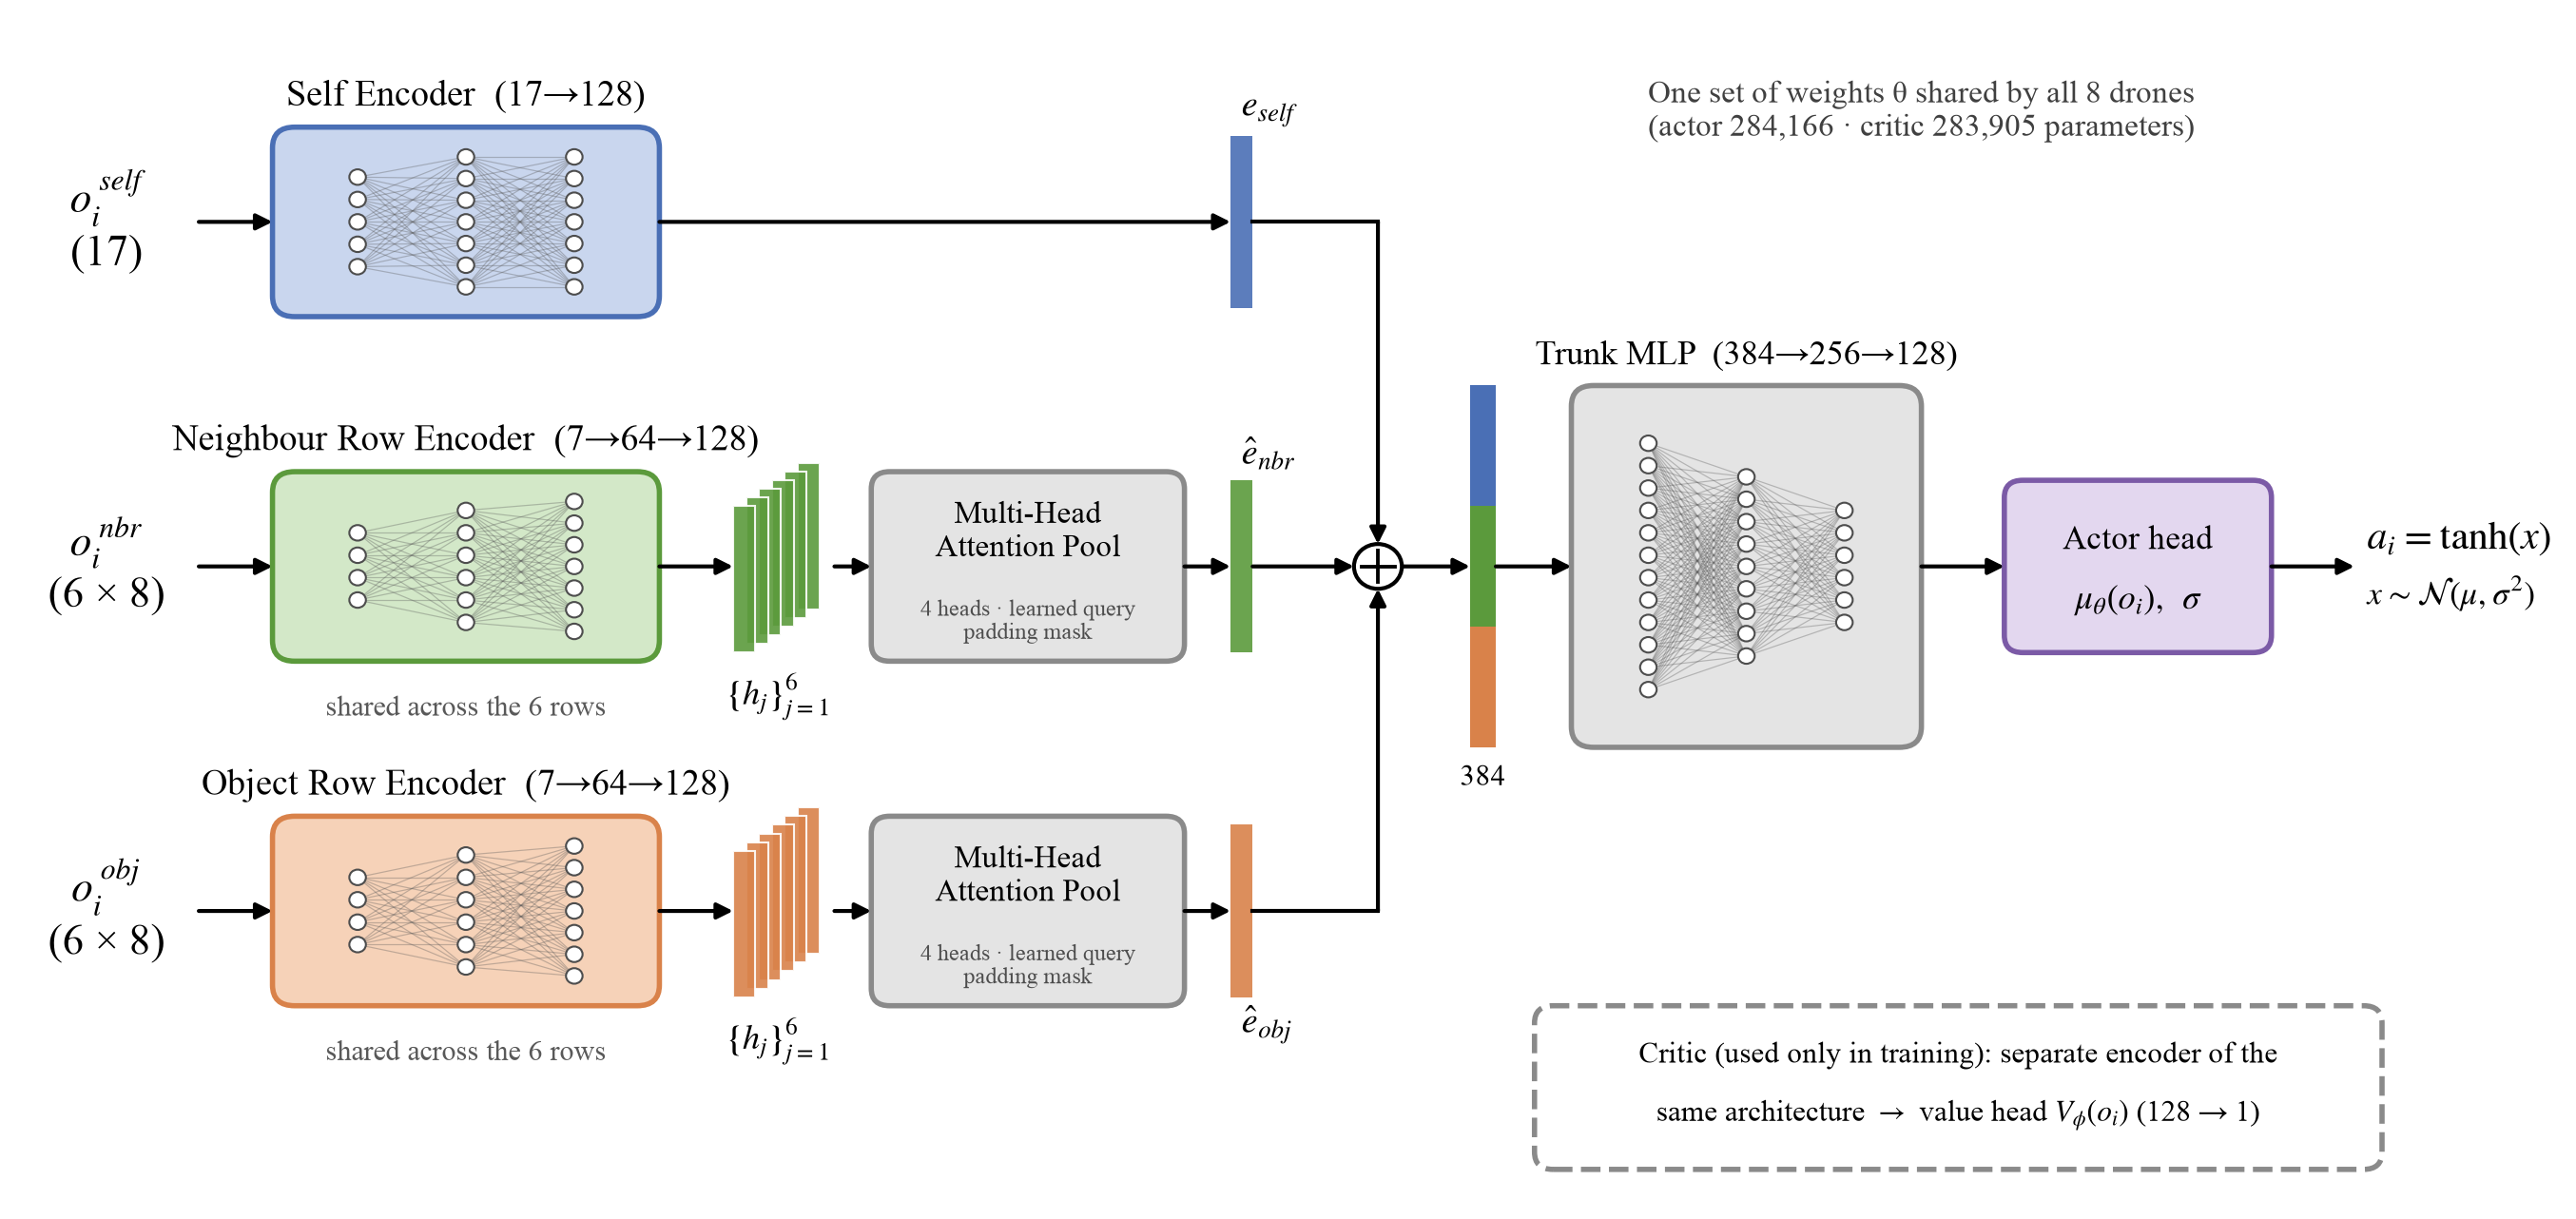
\includegraphics[width=0.9\textwidth]{fig_network_architecture}
  \caption[Architecture of the shared actor network]{Architecture of the shared actor network. Neighbour and
  object rows are encoded by shared MLPs and pooled by masked multi-head attention with a learned query; the
  pooled embeddings are concatenated with the self embedding and mapped to a squashed Gaussian velocity
  action.}
  \label{fig:network}
\end{figure}

\section{Learning Algorithm}
\subsection{Demonstration-guided initialisation}
At the beginning of every curriculum stage the actor is initialised by imitation of a sampling-based
model-predictive expert planner. The planner uses the same local observation; it simulates 86 candidate
velocity commands for 2\,s with the drone's response model, assumes that observed bodies keep their velocity,
and selects the command with the lowest cost for slot tracking and for violating soft (0.6\,m) and hard
(0.25\,m) clearance margins. In round 0 the expert flies with Gaussian action noise ($\sigma = 0.3$) while its
clean actions are recorded (noise-injected demonstrations, often called DART); in rounds 1--3 the current policy flies and the expert
labels every visited state (DAgger \cite{ross2011reduction}). After each round the actor is refit on all data
collected so far by minimising
\begin{equation}
  \mathcal{L}_{\mathrm{BC}}(\theta) = \mathbb{E}_{(o,a^\ast)\sim\mathcal{D}}
  \bigl\lVert \tanh\bigl(\mu_\theta(o)\bigr) - a^\ast \bigr\rVert^2 .
  \label{eq:bc}
\end{equation}

\subsection{Proximal policy optimisation}
The policy is then fine-tuned with PPO \cite{schulman2017proximal}. With the probability ratio
$\rho_t(\theta) = \pi_\theta(a_t\mid o_t)/\pi_{\theta_{\mathrm{old}}}(a_t\mid o_t)$, the clipped surrogate is
\begin{equation}
  \mathcal{L}^{\mathrm{CLIP}}(\theta) = -\,\mathbb{E}_t\Bigl[\min\bigl(\rho_t\hat A_t,\;
  \operatorname{clip}(\rho_t, 1-\epsilon, 1+\epsilon)\,\hat A_t\bigr)\Bigr],\qquad \epsilon = 0.2 .
  \label{eq:ppo}
\end{equation}
Advantages are estimated with GAE \cite{schulman2016gae} ($\gamma = 0.99$, $\lambda = 0.95$):
\begin{equation}
  \delta_t = r_t + \gamma\,(1-d_t)\,V_\phi(o_{t+1}) - V_\phi(o_t), \qquad
  \hat A_t = \delta_t + \gamma\lambda\,(1 - e_t)\,\hat A_{t+1},
  \label{eq:gae}
\end{equation}
where $d_t = 1$ only for a failure and $e_t = 1$ at any episode end; at the 24\,s time limit the value of the
final observation is bootstrapped instead of treated as terminal. The complete loss keeps
a decaying imitation term on the expert data, so that the demonstrated behaviour is retained during fine-tuning:
\begin{equation}
  \mathcal{L}(\theta,\phi) = \mathcal{L}^{\mathrm{CLIP}}(\theta) + 0.5\cdot\tfrac{1}{2}\,\mathbb{E}_t\bigl[(V_\phi(o_t)-\hat R_t)^2\bigr]
  + \beta(f)\,\mathcal{L}_{\mathrm{BC}}(\theta), \qquad \beta(f) = 1.0 - 0.5f,
  \label{eq:loss}
\end{equation}
where $\hat R_t = \hat A_t + V_\phi(o_t)$ and $f\in[0,1]$ is the progress within the stage. Rewards are divided
by a running standard deviation of the discounted return, advantages are normalised, actor and critic
gradients are clipped separately to norm 0.5, the learning rate is annealed linearly to 10\% of its initial
value, and the remaining epochs of an update are skipped when the mean approximate KL divergence of an epoch
exceeds 0.03. Before the first actor update, ten critic-only updates
prepare the value function for the imitation-initialised policy. In the obstacle stages, an episode that ends
in a collision is restored from a snapshot taken a few seconds earlier (at most twice per episode) and continued
with fresh on-policy steps, following the replay idea of \cite{huang2024collision}.

\subsection{Curriculum and model selection}
Training proceeds in three stages of increasing difficulty (a curriculum); each stage keeps the
scenarios of the previous stages and starts from the previous stage's best checkpoint. Every 100{,}000
environment steps the deterministic policy is validated on 10 selection seeds per scenario, and the checkpoint
with the highest selection score
\begin{equation}
  S = \overline{\text{success}} - 0.25\;\overline{\min(\text{RMSE}_{\mathrm{slot}}, 2)} - 0.25\,\bigl(1 - \text{recovered fraction}\bigr)
  \label{eq:score}
\end{equation}
is kept. Training, selection and final testing use disjoint seed ranges (0--999, 5000+, and 100000--100019
respectively), so that the reported test results are never used for tuning.

\section{Evaluation Metrics}
The formation error of an episode is the time-integrated slot RMSE,
\begin{equation}
  \text{RMSE}_{\mathrm{slot}} = \sqrt{\frac{1}{T_e}\sum_{t}\Delta t\,\frac{1}{N}\sum_{i=1}^{N}\lVert p_{i,t} - s_{i,t}\rVert^2 },
  \label{eq:rmse}
\end{equation}
where $T_e$ is the episode duration. A disturbance is \emph{recovered} when, after the object has left the
scene, every drone is simultaneously within 0.35\,m of its own slot and within 0.35\,m/s of the target
velocity for a continuous 1\,s; the recovery time includes this 1\,s confirmation. The minimum surface
clearance over the episode and the fraction of episodes completed without failure complete the evaluation.

\chapter{System Design and Implementation}
\label{ch:implementation}

\section{Software Architecture}
SwarmFlow is an independent Python~3.12 package built on the open-source libraries NumPy, Gymnasium, PettingZoo
and PyTorch. Simulation, learning, evaluation and
visualisation are separated into the modules listed in Table~\ref{tab:modules}. The environment implements the
PettingZoo parallel API: \texttt{reset} returns one observation per drone, and \texttt{step} receives one
action per drone and returns per-drone observations, rewards, termination and truncation flags. The simulator
state can be captured and restored, which is used for collision-state replay. The package is covered by 40
automated unit tests (all passing), including checks of swept collisions at high speed, immutable slot
assignment, recovery timing, reward bounds, attention permutation invariance, squashed-Gaussian
log-probabilities and time-limit handling in GAE.

\begin{table}[htbp]
\centering
\caption{Modules of the SwarmFlow implementation}
\label{tab:modules}
\small
\begin{tabularx}{\textwidth}{@{}lX@{}}
\toprule
Module & Responsibility\\
\midrule
\texttt{config.py}, \texttt{scenarios.py} & environment defaults; target paths, crossing-object generator, formation geometries, seeded scenarios\\
\texttt{env.py} & \texttt{SwarmEnv}: flight model, local observations, swept collisions, reward, recovery and episode metrics\\
\texttt{policy.py} & set encoders, shared actor--critic network, checkpoint loading for inference\\
expert planner & sampling-based model-predictive planner used to generate demonstrations\\
\texttt{train.py} & DART/DAgger imitation, parallel rollouts, reward scaling, GAE, PPO update, validation\\
\texttt{curriculum.py} & three-stage resumable training pipeline and held-out test of the selected model\\
\texttt{evaluate.py}, \texttt{suite.py} & episode runner, aggregate metrics, selection score and acceptance criteria\\
\texttt{server.py}, \texttt{web/} & local HTTP server and browser flight laboratory (HTML, JavaScript canvas)\\
\texttt{cli.py} & command-line entry points \texttt{view}, \texttt{eval}, \texttt{train}, \texttt{pipeline}\\
\bottomrule
\end{tabularx}
\end{table}

\section{Training Pipeline}
Figure~\ref{fig:curriculum} shows the complete training pipeline. Stage~1 learns formation keeping with a
static, moving and turning target; stage~2 adds lateral and head-on objects; stage~3 adds repeated crossings
and the wind gust. Inside every stage, four demonstration rounds (one DART round and three DAgger rounds) are
followed by validation of the initialised policy, ten critic warm-up updates and PPO fine-tuning. Rollouts are
collected from eight environment instances whose neural-network inference is batched: each update uses
$8 \times 256 \times 8 = 16{,}384$ drone transitions. Every update writes a resumable checkpoint, so an
interrupted run continues where it stopped.

\begin{figure}[htbp]
  \centering
  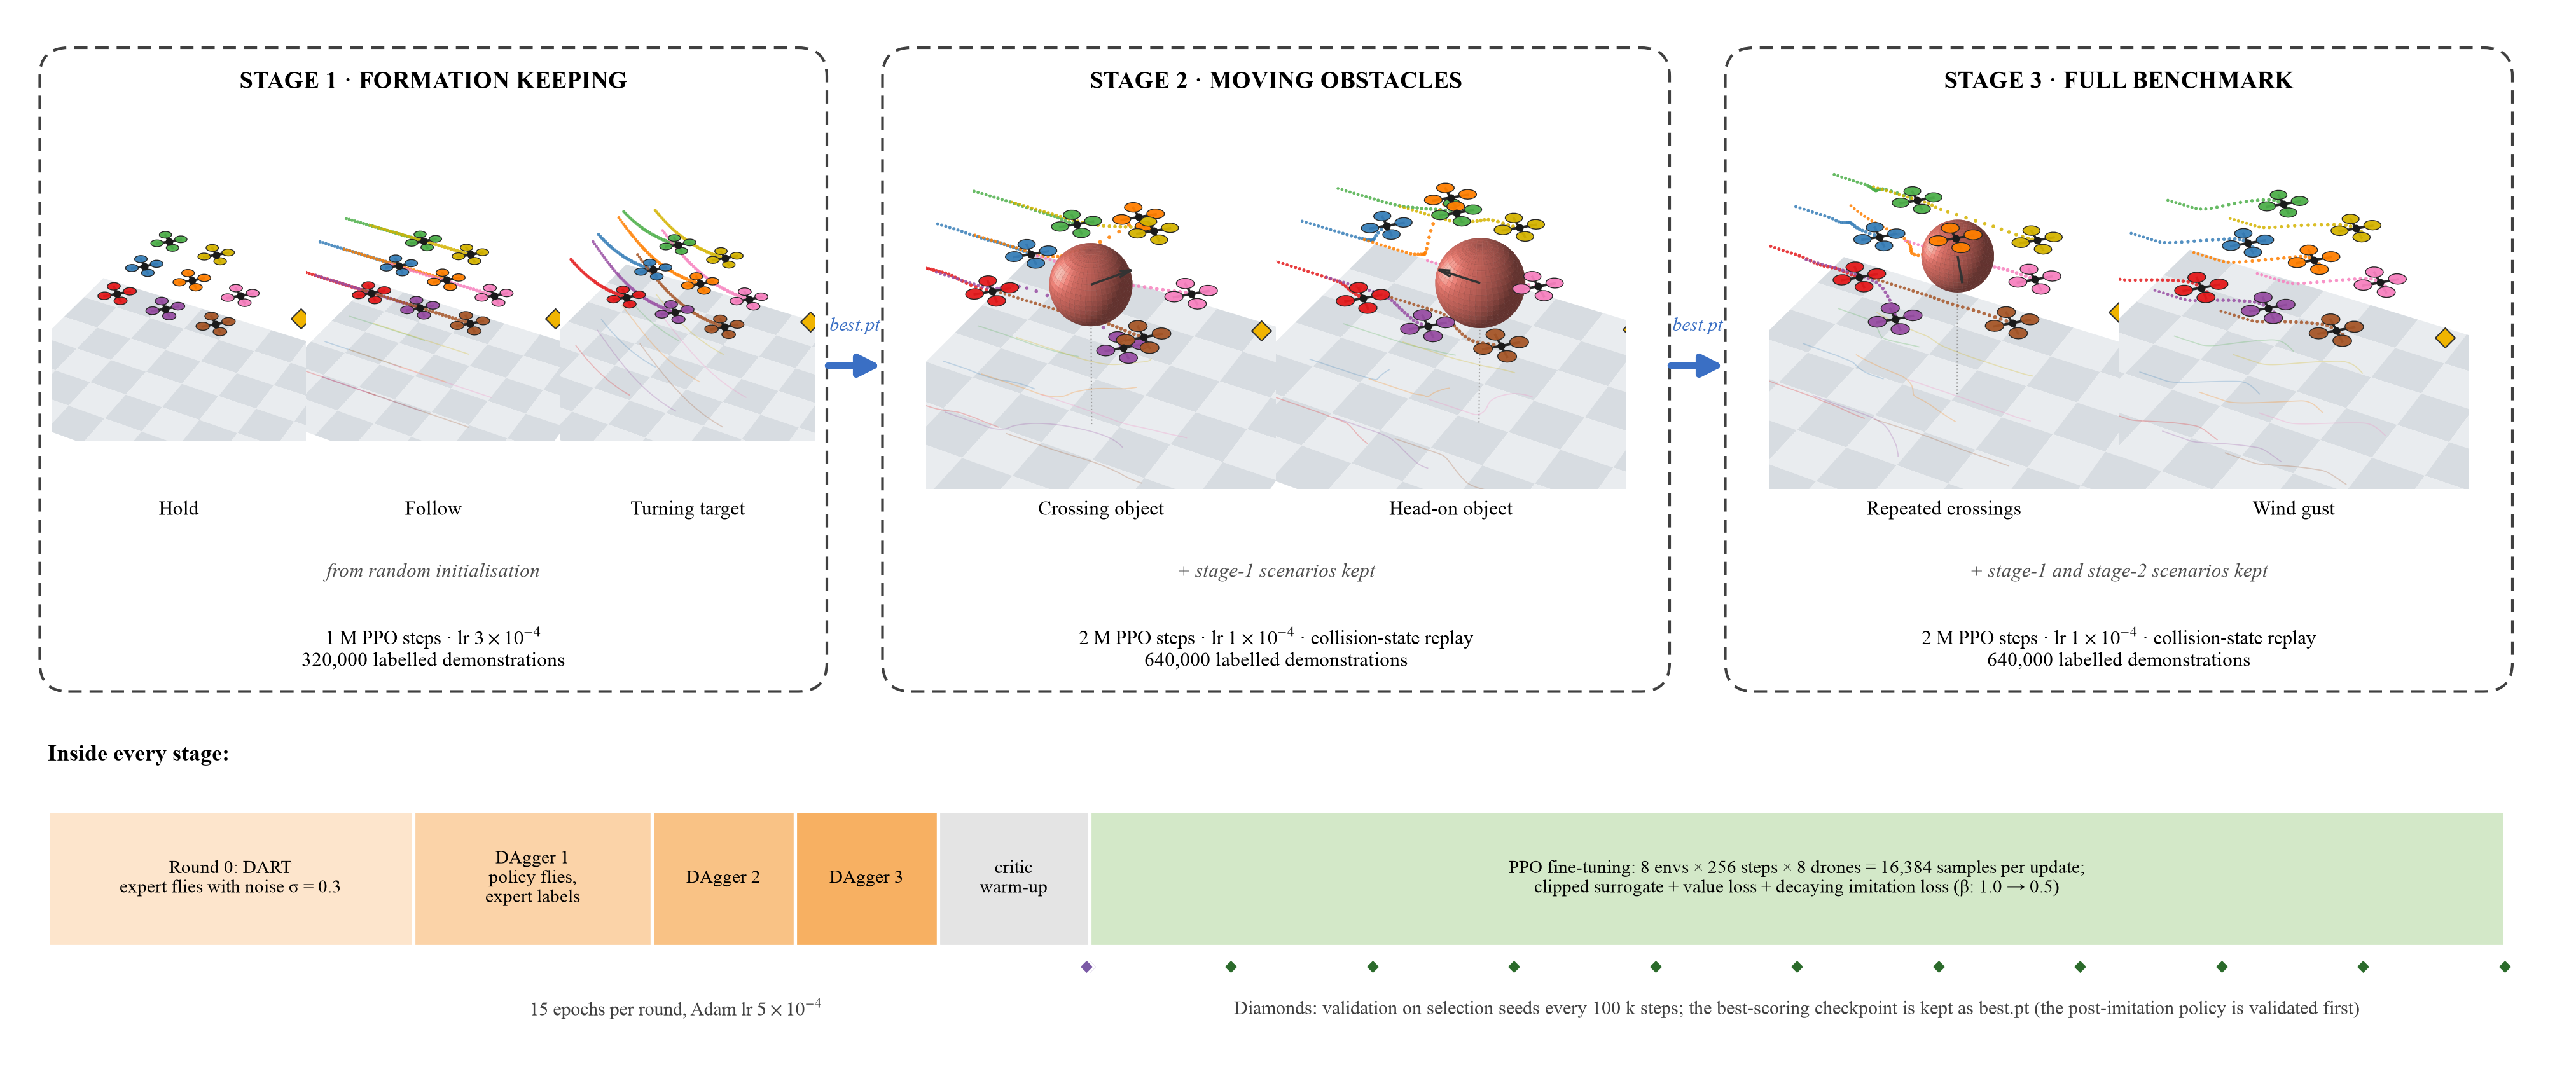
\includegraphics[width=0.88\textwidth]{fig_curriculum}
  \caption[Three-stage curriculum training pipeline]{Three-stage curriculum. Each stage adds harder scenarios
  (thumbnails rendered from the simulator), keeps the earlier ones and starts from the best checkpoint of the
  previous stage. The bar shows the phases inside every stage.}
  \label{fig:curriculum}
\end{figure}

\section{Training Configuration}
Table~\ref{tab:hyper} lists the configuration of the final model. The complete PPO budget is
$5\times10^{6}$ environment steps, i.e.\ $4\times10^{7}$ individual drone decisions. The PPO phases of the
three stages took 1{,}925\,s, 3{,}904\,s and 3{,}999\,s (about 2.7\,h in total) on a laptop at roughly
550--570 environment steps per second.

\begin{table}[htbp]
\centering
\caption{Training configuration of the final model}
\label{tab:hyper}
\footnotesize
\setlength{\tabcolsep}{4pt}
\begin{tabular}{@{}llll@{}}
\toprule
Setting & Value & Setting & Value\\
\midrule
PPO steps (stage 1/2/3) & 1\,M / 2\,M / 2\,M & Learning rate (stage 1 / 2--3) & $3\!\times\!10^{-4}$ / $1\!\times\!10^{-4}$\\
Parallel environments & 8 & Rollout horizon & 256 steps\\
Samples per update & 16{,}384 & Epochs / minibatch & 5 / 2{,}048\\
Discount $\gamma$ / GAE $\lambda$ & 0.99 / 0.95 & Clip $\epsilon$ / KL limit & 0.2 / 0.03\\
Initial / minimum action std & 0.20 / 0.05 & Entropy coefficient & 0\\
Imitation weight $\beta$ & 1.0 $\to$ 0.5 & Gradient clip (actor, critic) & 0.5, 0.5\\
Demonstration rounds & 4 (15 epochs each) & Demonstration steps per round & 10\,k (stage 1), 20\,k\\
Labelled samples (stage 1/2/3) & 320\,k / 640\,k / 640\,k & Expert margins (soft / hard) & 0.6\,m / 0.25\,m\\
Validation & every 100\,k steps & Selection seeds & 10 per scenario\\
Optimiser & Adam, $\varepsilon = 10^{-5}$ & Network width & 128\\
\bottomrule
\end{tabular}
\end{table}

\section{Web-Based Flight Laboratory}
To demonstrate and inspect the learned behaviour, the project includes a browser-based flight laboratory
(Figure~\ref{fig:viewer}). A local Python server runs the simulation and exposes a small REST interface
(\texttt{/api/state}, \texttt{/api/reset}, \texttt{/api/step}, \texttt{/api/inject}); the page renders the
actual three-dimensional simulation state on an HTML canvas. The user can select the scenario, formation
geometry, number of drones and seed, start and pause a flight, orbit the camera or switch to side and top
projections, and inject additional crossing or head-on objects with chosen speed and radius at any time. Live
panels show the slot error, the minimum surface clearance, the number of recovered disturbances and the flight
state. A second panel reports the training history and the held-out test of the loaded model. The viewer only
executes the saved network weights; it does not modify them.

\begin{figure}[htbp]
  \centering
  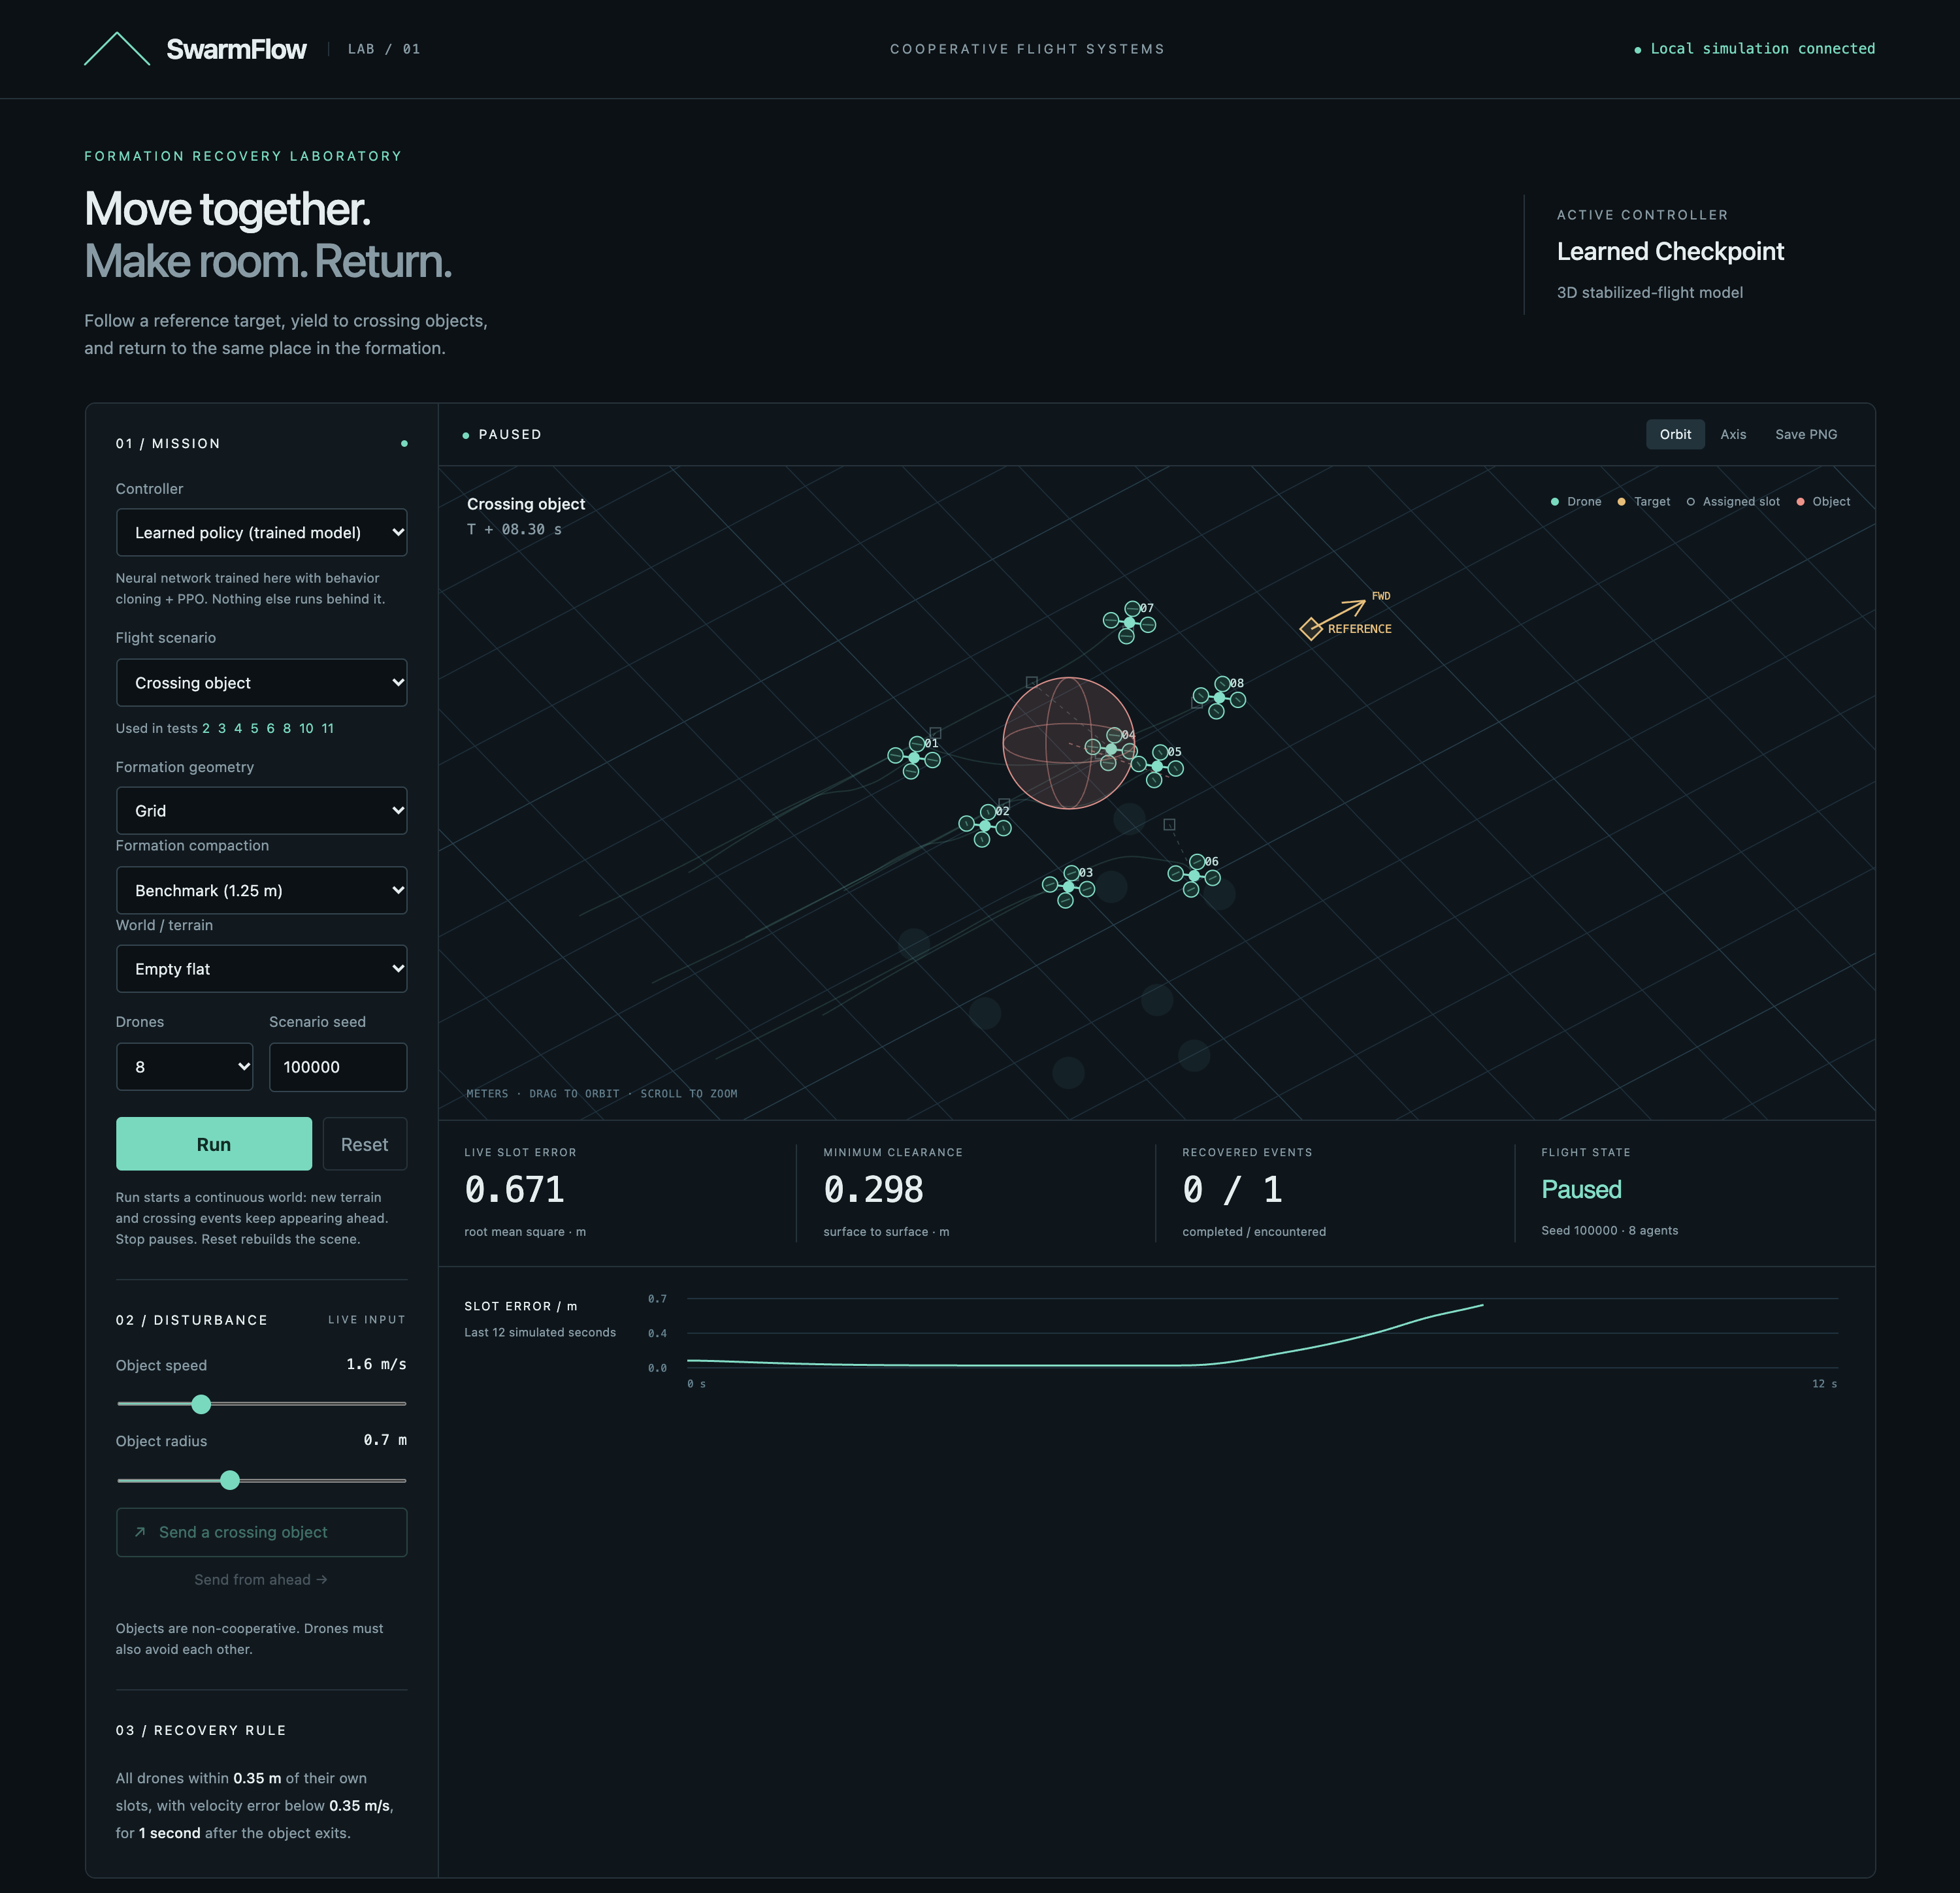
\includegraphics[width=0.6\textwidth]{viewer/viewer_overview}
  \caption[SwarmFlow web flight laboratory running the final model]{SwarmFlow web flight laboratory running the
  final model (crossing scenario, held-out seed 100000, $t = 8.3$\,s). Left: mission and disturbance controls;
  centre: 3-D view with drones (numbered), assigned slots (squares), reference target and object; bottom: live
  metrics and slot-error timeline.}
  \label{fig:viewer}
\end{figure}

\chapter{Results and Discussion}
\label{ch:results}

\section{Experimental Setup}
All results in this chapter were produced by the final trained model with the deterministic action
$a_i = \tanh(\mu_\theta(o_i))$ and no additional controller behind the network. The final evaluation uses the
seven benchmark scenarios with 20 held-out seeds each (seeds 100000--100019, never used for training or model
selection), i.e.\ 140 episodes of 24\,s with eight drones. The demonstrations in
Sections~\ref{sec:demo}--\ref{sec:disturbance} use held-out seed 100000; the three-dimensional renderings are
drawn from the recorded simulator states and the screenshots are taken from the running web flight laboratory
with the same configuration.

\section{Demonstration of the Final System}
\label{sec:demo}
Figure~\ref{fig:render_crossing} shows a complete \emph{follow, yield, recover} cycle for a lateral crossing
object. Before the object arrives the eight drones hold their grid slots while following the target (a). As the
object crosses the formation, the drones nearest to its path move out of the way, in three dimensions, while the
others keep their places (b). After the object has passed, every drone returns to its own slot; the dotted
trails show the avoidance manoeuvre and the transparent sphere marks the earlier object position (c). In this
episode the minimum surface clearance was 0.298\,m and the formation was recovered 1.51\,s after the object
left the scene.

\begin{figure}[htbp]
  \centering
  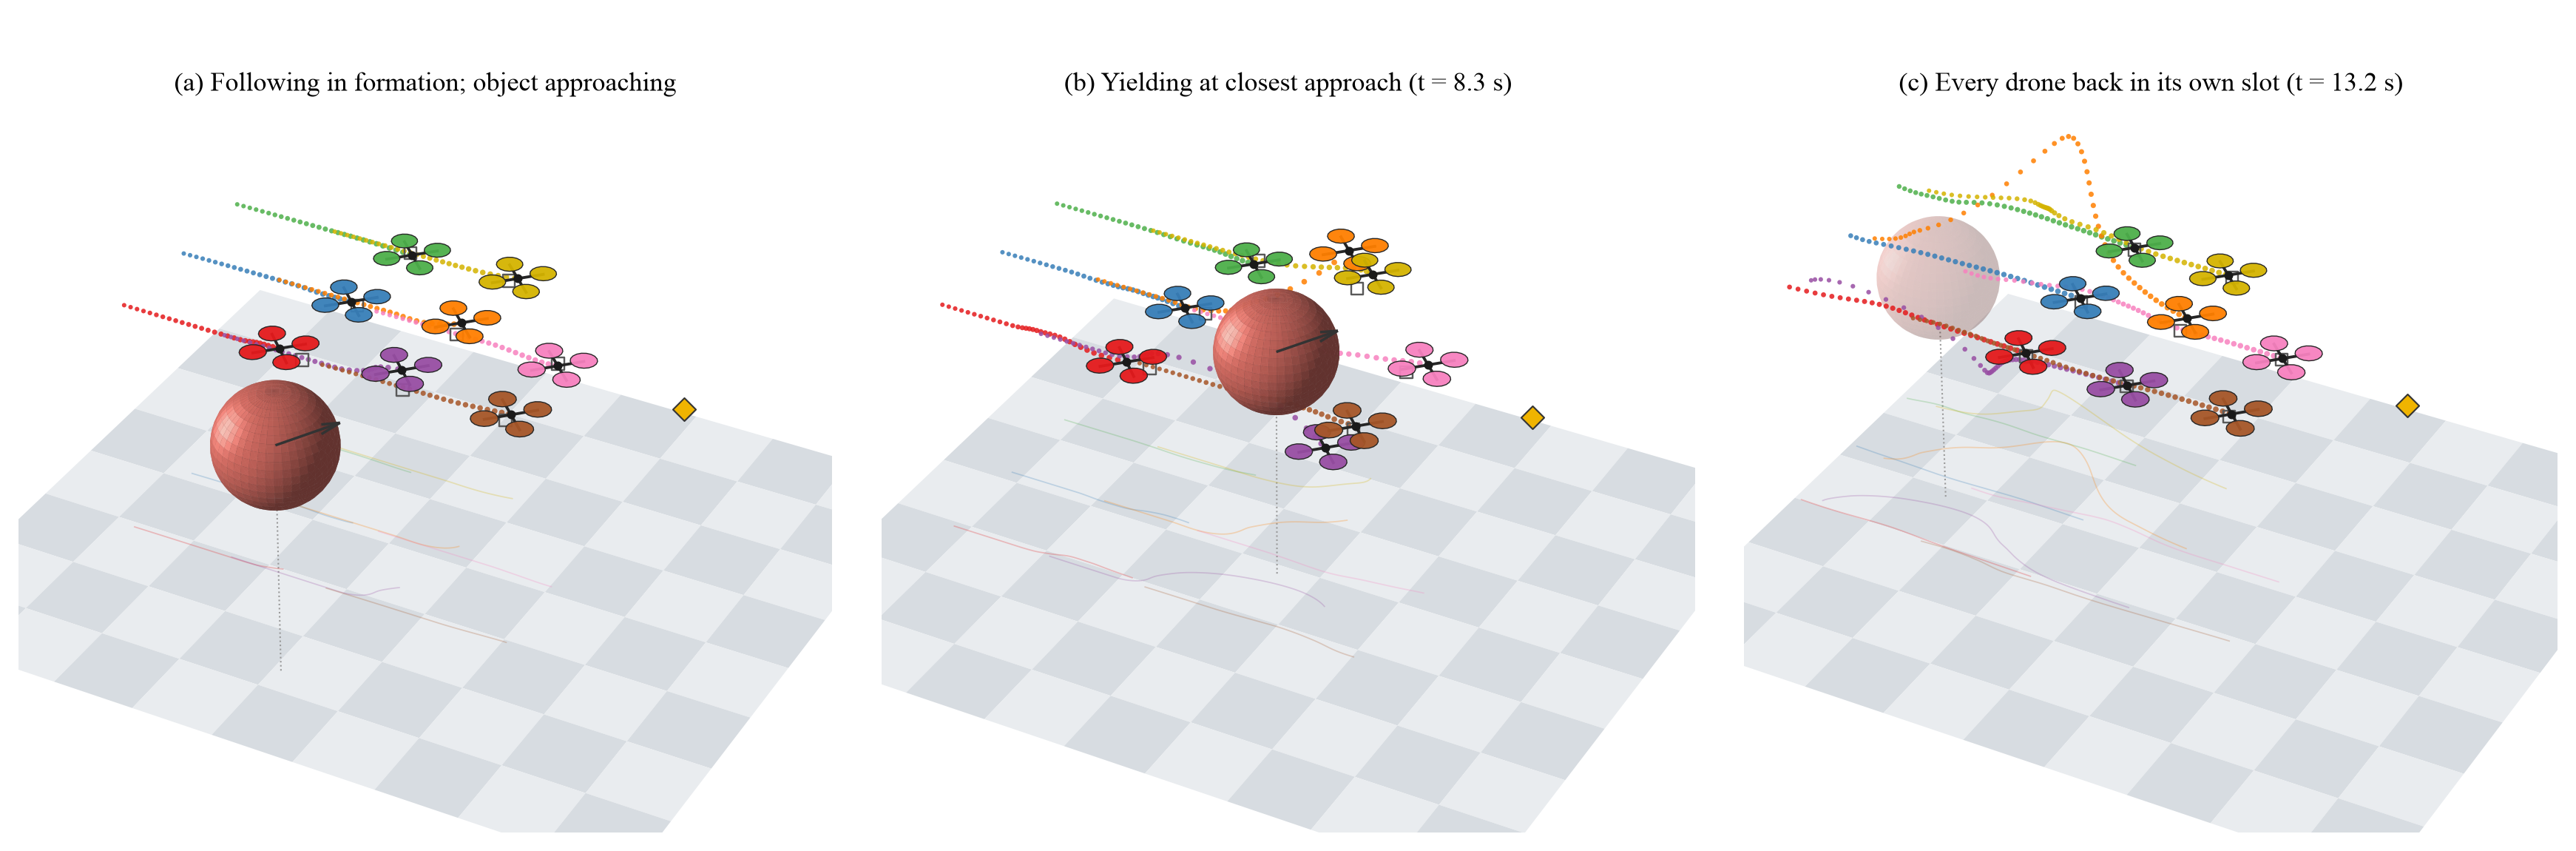
\includegraphics[width=0.95\textwidth]{fig_render_crossing}
  \caption[Follow, yield and recover behaviour of the final model]{Follow, yield and recover behaviour of the
  final model for a lateral crossing object (held-out seed 100000). Coloured quadrotors are the eight drones,
  dotted lines their trails, squares their assigned slots and the diamond the reference target.}
  \label{fig:render_crossing}
\end{figure}

The same episode in the web flight laboratory is shown in Figure~\ref{fig:viewer_sequence}. The live metrics
of the viewer agree with the offline evaluation, confirming that the demonstration is produced by the trained
network itself.

\begin{figure}[htbp]
  \centering
  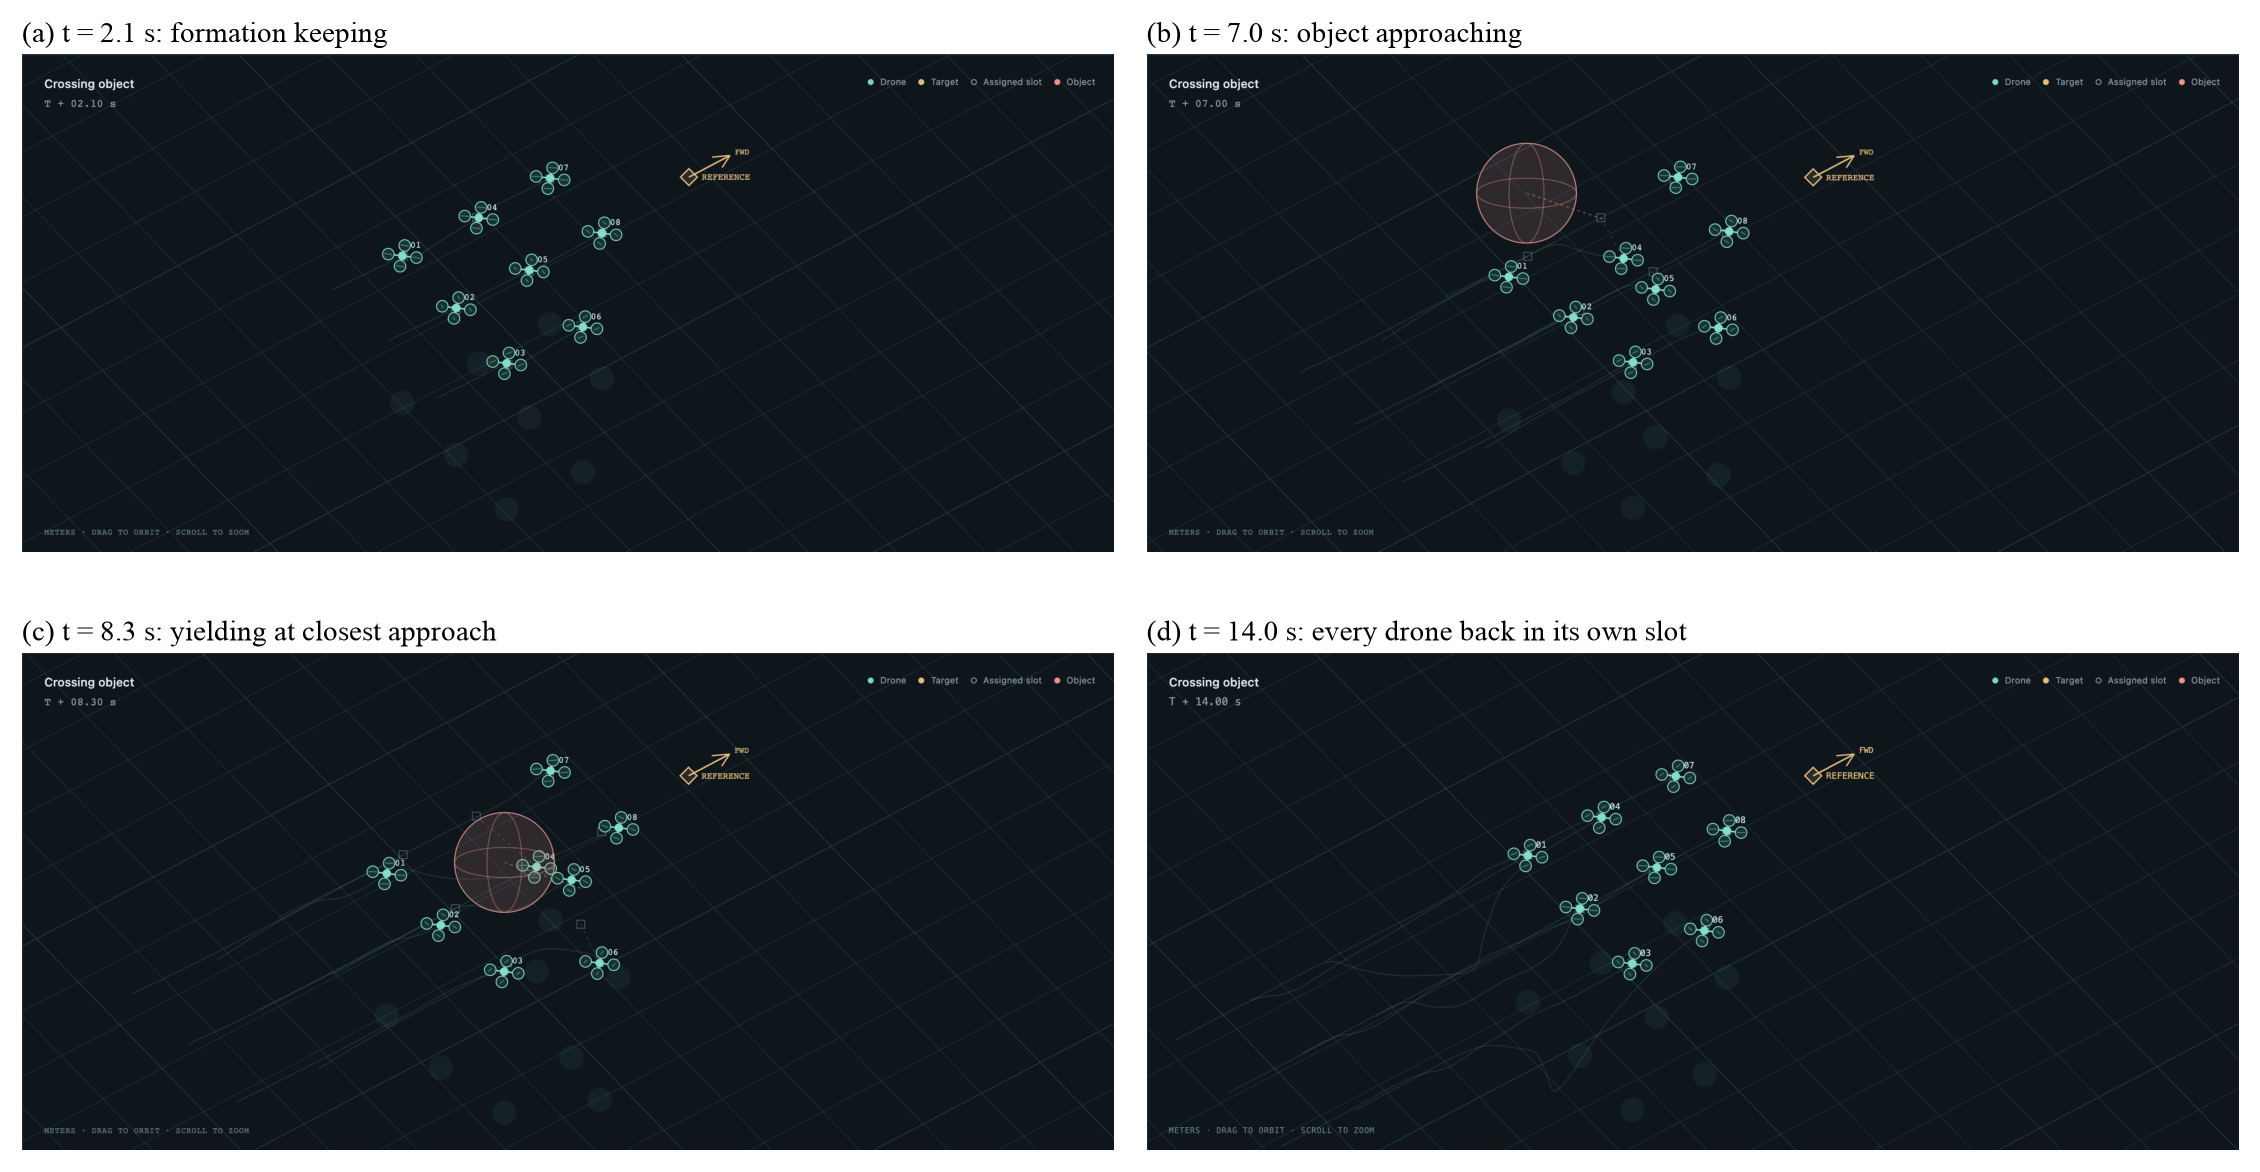
\includegraphics[width=0.76\textwidth]{fig_viewer_crossing_sequence}
  \caption[Crossing episode in the web flight laboratory]{The crossing episode of
  Figure~\ref{fig:render_crossing} in the SwarmFlow web flight laboratory: formation keeping (a), object
  approaching (b), yielding at closest approach (c) and complete recovery to the assigned slots (d).}
  \label{fig:viewer_sequence}
\end{figure}

Figure~\ref{fig:render_headon} shows the two more demanding disturbances. For a head-on object, which
approaches faster (relative speed 1.8--2.2\,m/s) and is larger, the formation opens around the object and
closes again, recovering 1.67\,s after the object left (a, b). In the repeated-crossing scenario a second
object arrives from the opposite side; the swarm yields again and recovers both disturbances, 1.51\,s and
2.00\,s after the respective exits (c).

\begin{figure}[htbp]
  \centering
  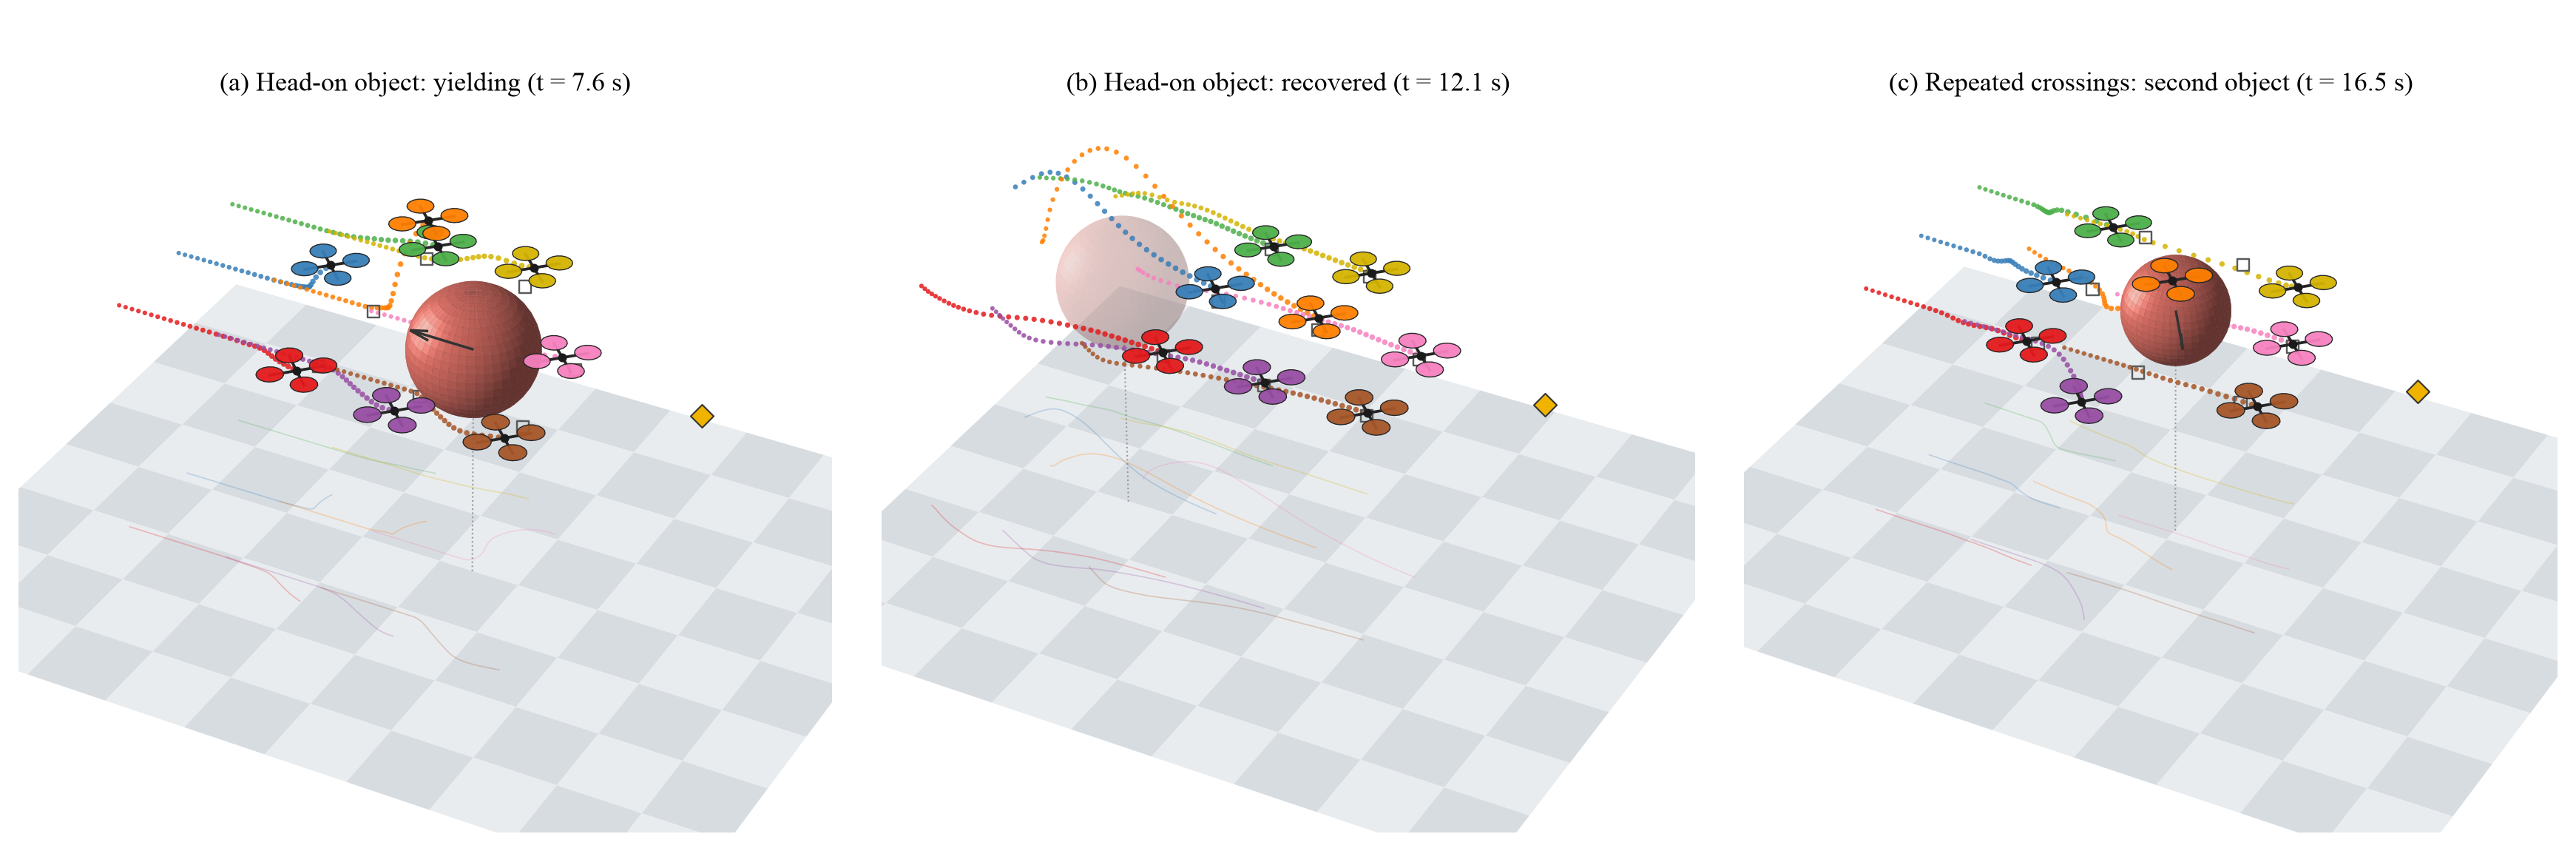
\includegraphics[width=0.95\textwidth]{fig_render_headon_double}
  \caption[Head-on and repeated-crossing behaviour]{Head-on object during yielding (a) and after recovery (b),
  and the second object of a repeated-crossing episode (c); held-out seed 100000.}
  \label{fig:render_headon}
\end{figure}

\section{Formation Disturbance and Recovery}
\label{sec:disturbance}
Figure~\ref{fig:timeseries} plots the distance of every drone to its own slot over time for the three disturbance
scenarios. Before the object arrives the error of all drones is only a few centimetres. During the object's
passage (shaded) only the drones close to its path deviate, by up to about 1.8\,m, and the swarm-level RMS error
returns below the 0.35\,m tolerance shortly after the object leaves. The green dashed lines mark the confirmed
recoveries; after recovery the formation error returns to its undisturbed level.

\begin{figure}[htbp]
  \centering
  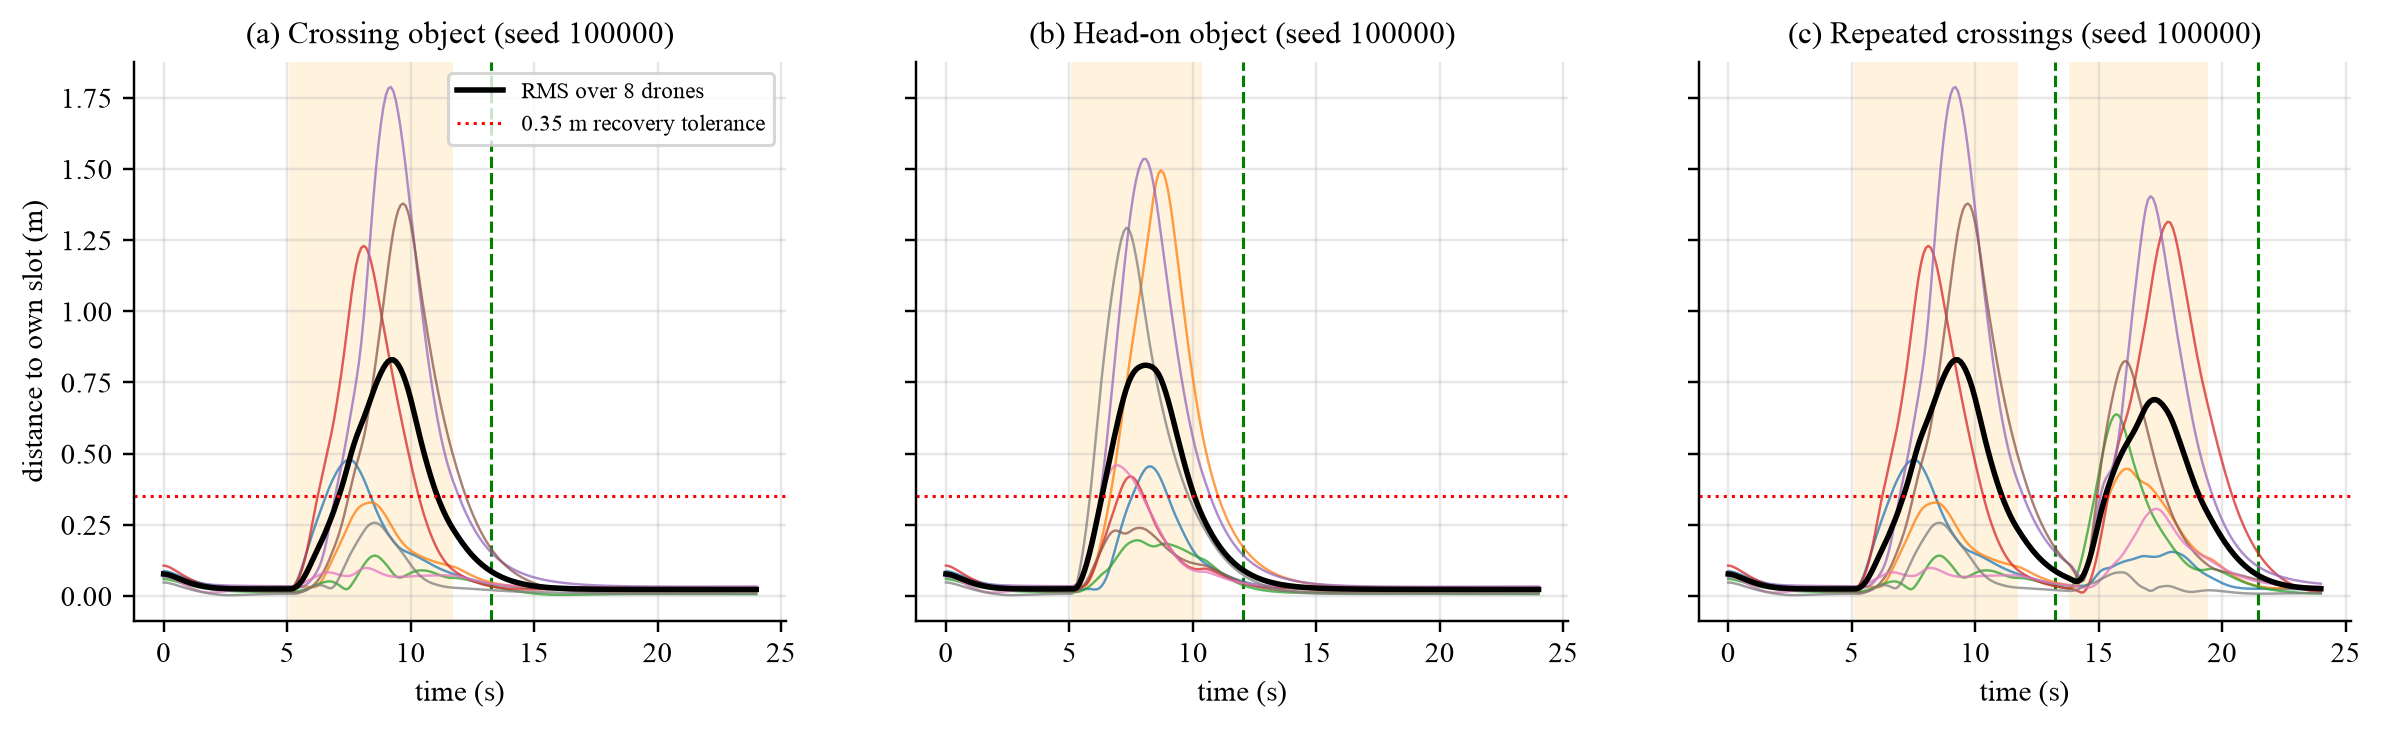
\includegraphics[width=0.9\textwidth]{fig_slot_error_timeseries}
  \caption[Distance of each drone to its own slot over time]{Distance of each drone to its own slot (thin
  lines) and RMS over the swarm (black) for held-out seed 100000. Shaded: object inside the scene; green dashed:
  confirmed recovery; red dotted: 0.35\,m recovery tolerance.}
  \label{fig:timeseries}
\end{figure}

\section{Held-Out Evaluation}
Table~\ref{tab:results} and Figure~\ref{fig:results} summarise the evaluation on the 140 held-out episodes.
The model completed 138 episodes (98.6\%) without failure and achieved 100\% success in six of the seven
scenarios. In the three undisturbed scenarios the formation error was 0.023\,m, 0.027\,m and 0.045\,m, well
below the 0.35\,m criterion; the wind gust increased it only to 0.176\,m. All 78 disturbances in the completed
episodes were recovered, 70 of all 80 within 5\,s; the mean recovery time was 1.9\,s for crossing and 2.4\,s for
head-on objects. In the head-on scenario 18 of 20 episodes were completed; in the remaining two, a drone made brief
contact with the object while passing it (minimum clearance $-0.04$\,m), which identifies the
head-on case as the main target for the further improvements described in Section~\ref{sec:future}.
Measured against the three criteria of Section~\ref{sec:problem}, the formation-precision criterion is met in every
undisturbed scenario, 98.6\% of the episodes are collision-free, and 87.5\% of the disturbances are recovered
within 5\,s; the remaining cases are concentrated in the head-on and double-crossing scenarios.

\begin{table}[htbp]
\centering
\caption{Held-out evaluation of the final model (20 unseen seeds per scenario)}
\label{tab:results}
\small
\begin{tabular}{@{}lccccc@{}}
\toprule
Scenario & Episodes & Slot RMSE & Disturbances & Mean / max & Min.\ surface\\
 & completed & (m) & recovered & recovery (s) & clearance (m)\\
\midrule
Hold             & 20/20 & 0.023 & -- & -- & 0.764\\
Follow           & 20/20 & 0.027 & -- & -- & 0.764\\
Turning target   & 20/20 & 0.045 & -- & -- & 0.764\\
Wind gust        & 20/20 & 0.176 & -- & -- & 0.764\\
Crossing         & 20/20 & 0.274 & 20/20 & 1.88 / 3.07 & 0.183\\
Head-on          & 18/20 & 0.289 & 18/20 & 2.43 / 4.12 & $-0.041$\\
Double crossing  & 20/20 & 0.393 & 40/40 & 3.47 / 11.36 & 0.009\\
\midrule
Total            & 138/140 & -- & 78/80 & -- & --\\
\bottomrule
\end{tabular}
\end{table}

\begin{figure}[htbp]
  \centering
  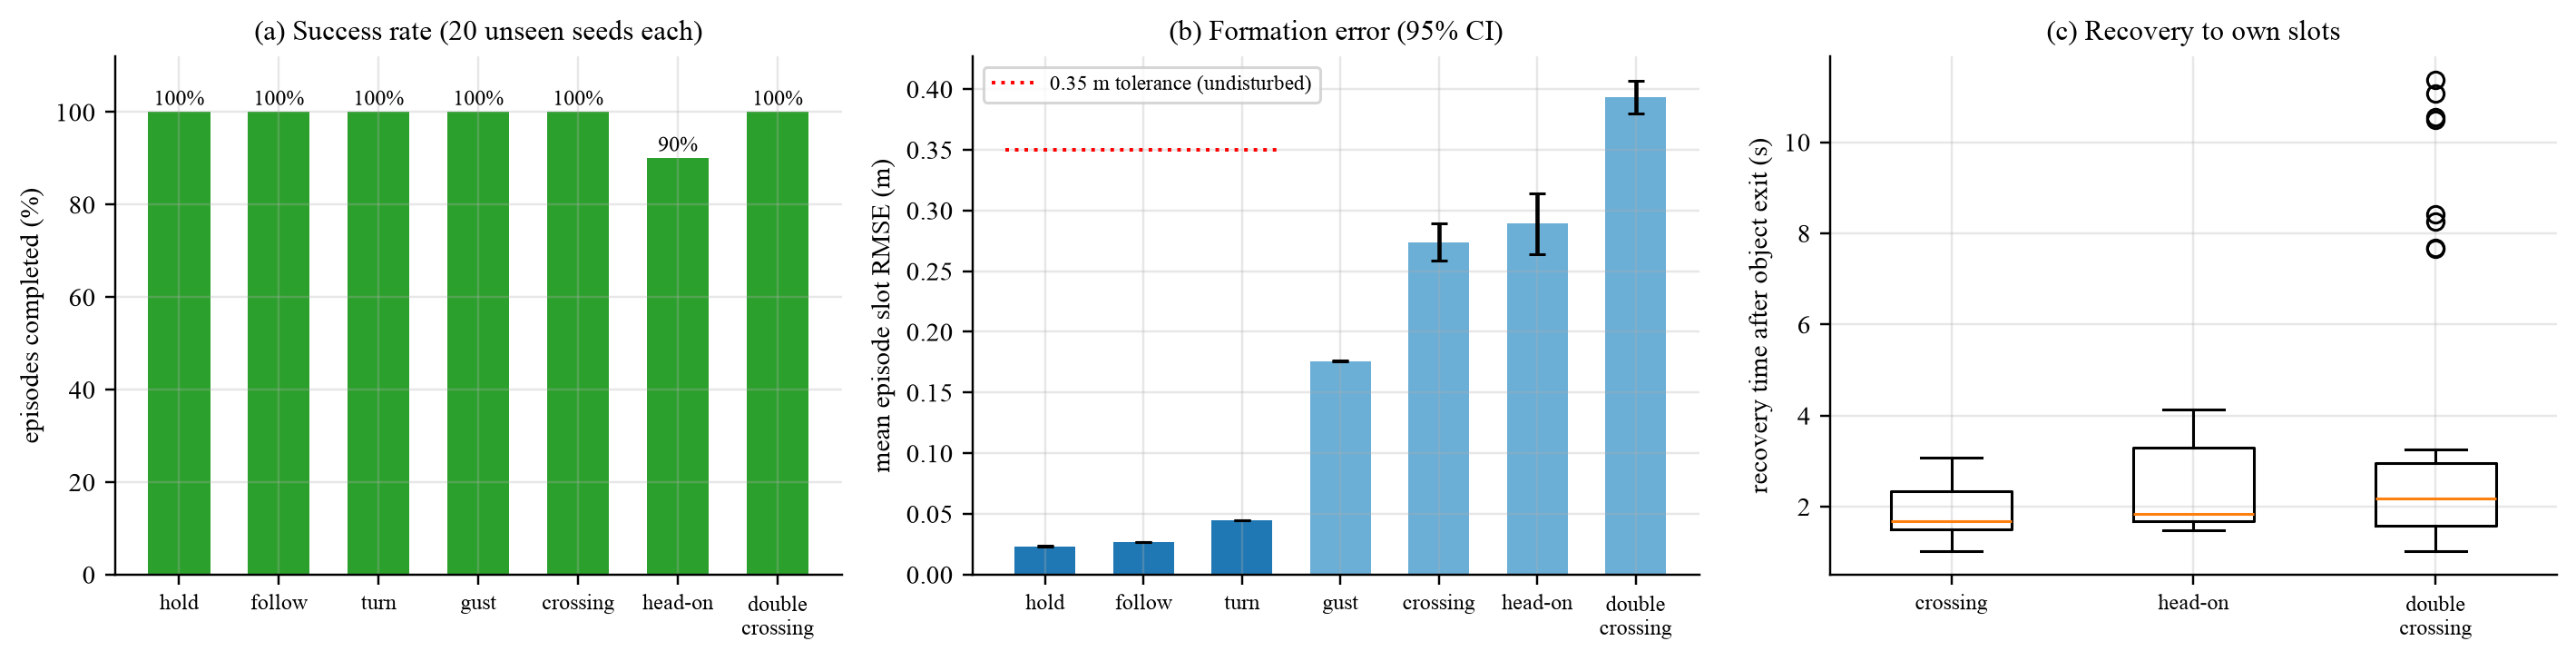
\includegraphics[width=0.9\textwidth]{fig_results_scenarios}
  \caption[Held-out success rate, formation error and recovery time]{Held-out evaluation of the final model:
  (a) episodes completed without failure, (b) mean episode slot RMSE with 95\% confidence intervals, and
  (c) recovery time after each object exit.}
  \label{fig:results}
\end{figure}

In the double-crossing scenario the second object sometimes enters while the swarm is still settling from the
first; the recovery clock of the first event then includes the second passage, which explains the few longer
recovery times in Figure~\ref{fig:results}(c).

\section{Training Behaviour}
Figure~\ref{fig:imitation}(a) shows the imitation error after each of the four demonstration rounds of every
stage: the action error decreases steadily (in stage~1 from $1.6\times10^{-3}$ to $4.0\times10^{-4}$) as DAgger
adds the states visited by the learner itself. During stage-1 PPO the formation error of the training episodes
fell from about 0.21\,m to below 0.06\,m (b), without a single training failure.

\begin{figure}[htbp]
  \centering
  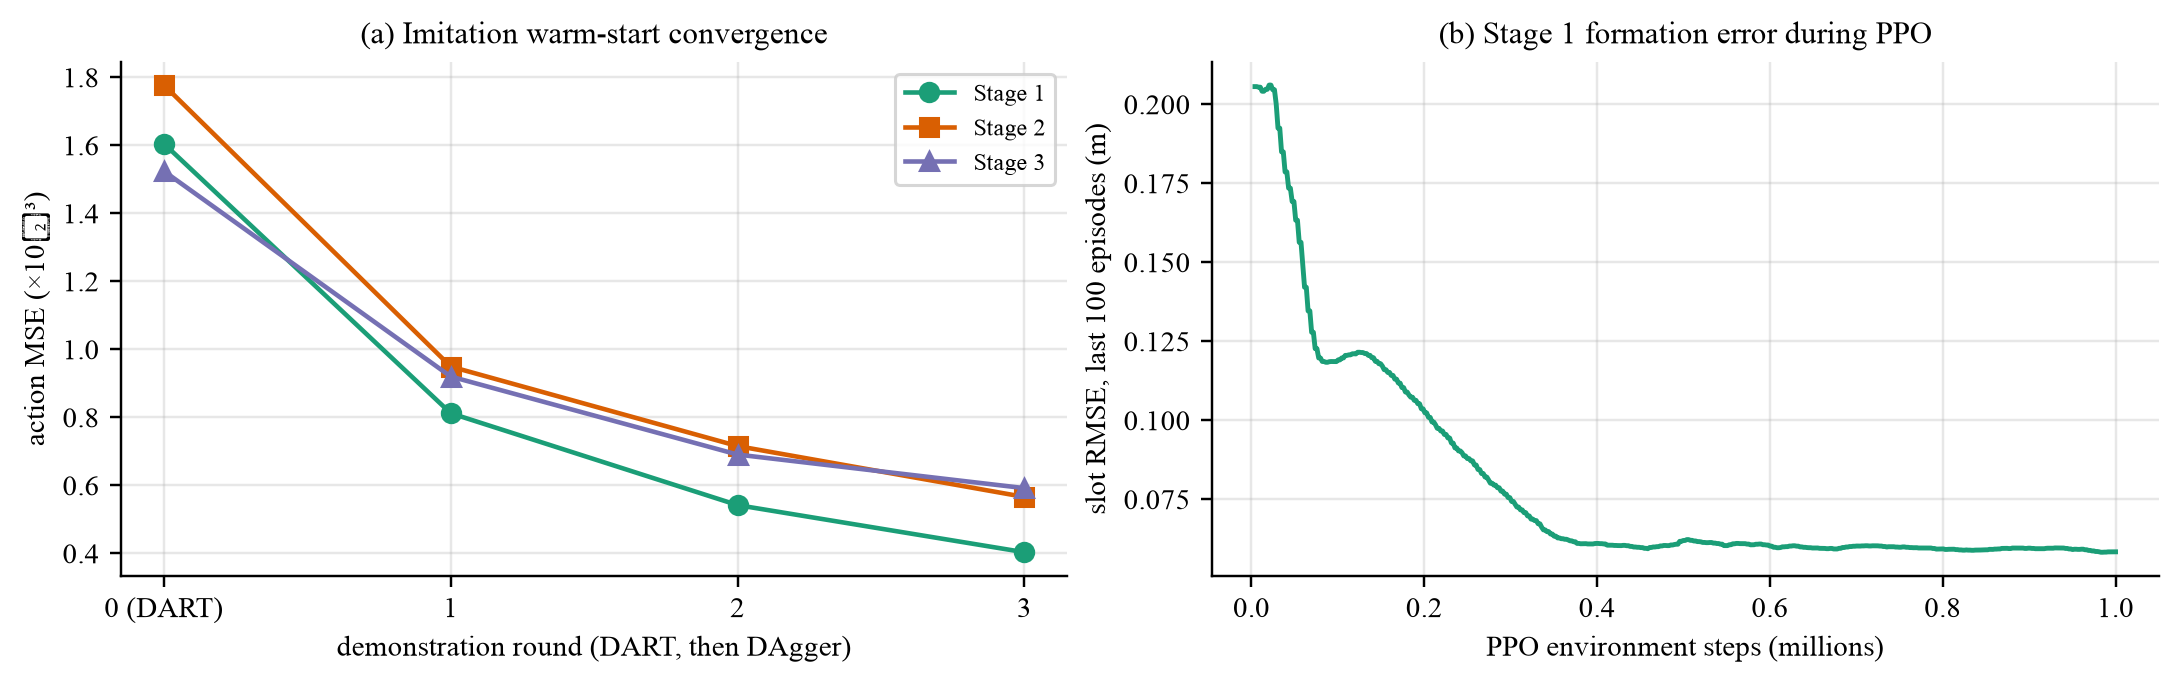
\includegraphics[width=0.85\textwidth]{fig_imitation_and_stage1}
  \caption[Imitation convergence and stage-1 training error]{(a) Action MSE after each demonstration round of
  the three stages. (b) Slot RMSE of the last 100 training episodes during stage-1 PPO.}
  \label{fig:imitation}
\end{figure}

Figure~\ref{fig:training_panel} shows the full
training history as reported by the web flight laboratory. The validation score stays close to 1.0 in stage~1;
in stages~2 and~3 the harder scenarios make the score vary between validations, and model selection retains
the best checkpoint of each stage (validation scores 0.997, 0.968 and 0.957). The selected final model reached
a held-out score of 0.936 on the unseen test seeds, close to its validation score, which indicates that it
generalises to new scenario instances.

\begin{figure}[htbp]
  \centering
  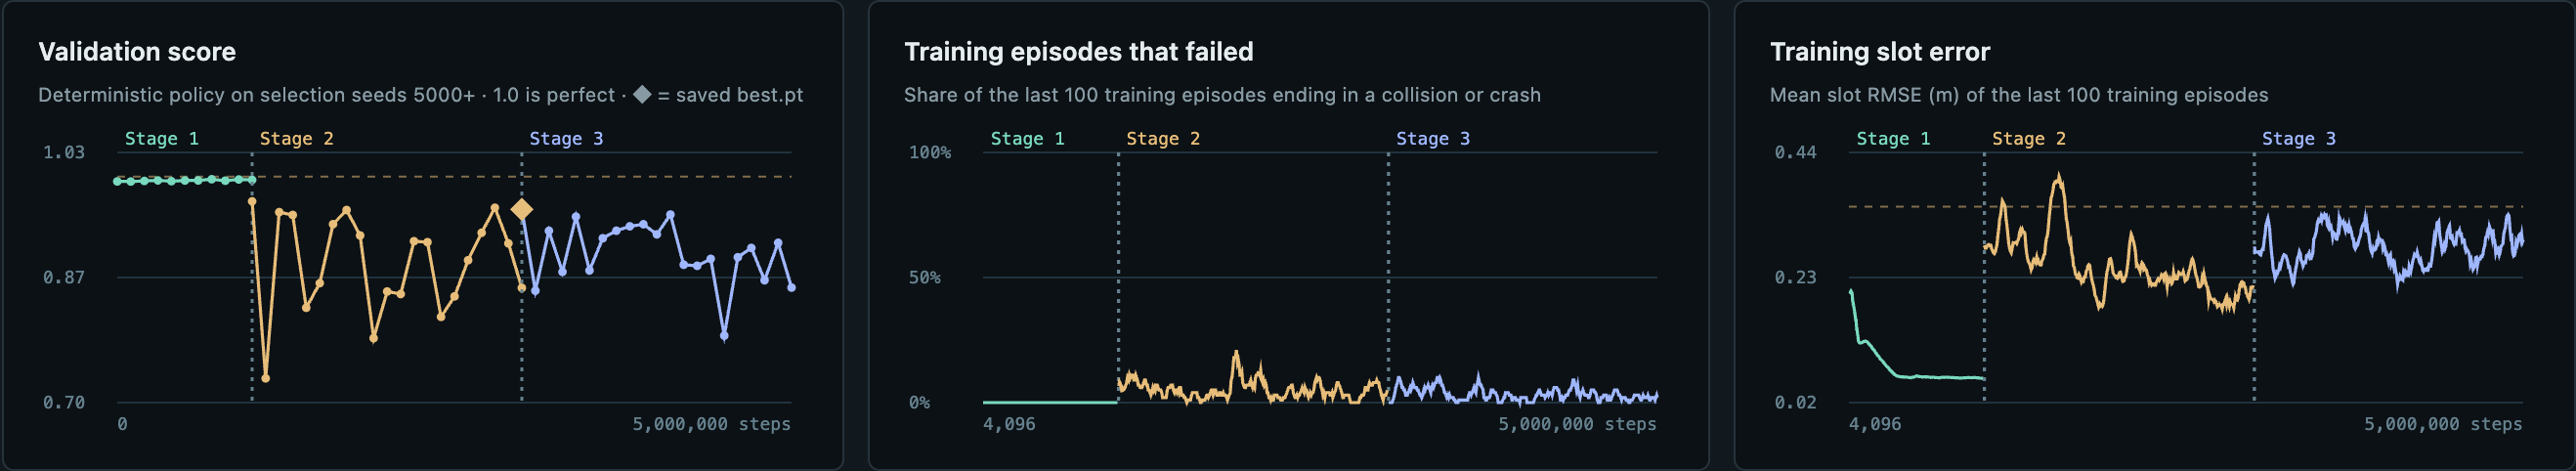
\includegraphics[width=0.9\textwidth]{viewer/model_training_charts}
  \caption[Training history of the final model in the flight laboratory]{Training history of the final model
  over the three-stage curriculum as displayed by the web flight laboratory: validation score (diamond: selected
  checkpoint), share of failed training episodes and training slot error.}
  \label{fig:training_panel}
\end{figure}

\section{Ongoing Development}
After the final model had been validated, a revised training configuration (version~4) was prepared. It enlarges
the clearance margins of the expert planner in the demonstration data (0.7\,m / 0.3\,m), refines the recovery
measurement when two disturbances overlap, and shortens the fine-tuning budget of stages~2 and~3 to 1\,M PPO
steps. This version was trained on a separate team machine: its first stage completed with a validation score
of 0.996, but errors were observed in the output during the subsequent training phase and the run was not
completed. The model presented in this report (version~3) therefore remains the final validated system, and the
completion of the version-4 training is part of the future work.

\section{Task, Achievement and Possible Beneficiaries}
The task of this project was to learn a decentralised controller that lets a drone swarm follow a target, yield
to moving objects and recover its formation. The achieved system meets the formation-precision criterion in all
undisturbed scenarios, completes 98.6\% of the held-out episodes without failure, returns every drone to its own
slot after every disturbance in the completed episodes, and runs as an interactive demonstration in which new
objects can be injected during flight. The approach and software can benefit:
\begin{itemize}
  \item researchers in multi-agent reinforcement learning and swarm robotics, as a compact and reproducible
        benchmark with explicit recovery metrics;
  \item developers of drone-show, inspection and surveillance systems that require formation flight in shared
        airspace;
  \item educators, through the interactive flight laboratory that visualises learned multi-agent behaviour.
\end{itemize}

\section{Review of Contributions}
\begin{enumerate}
  \item A PettingZoo multi-agent environment for formation following, yielding and same-slot recovery with a
        stabilised flight model and continuous swept collision detection.
  \item A bounded, per-drone reward with culprit-only failure penalties and a quantitative recovery criterion.
  \item A shared, permutation-invariant actor--critic network with masked multi-head attention pooling over
        neighbours and objects.
  \item A three-stage curriculum combining DART and DAgger initialisation from an expert planner with PPO and
        GAE fine-tuning, collision-state replay and validation-based model selection.
  \item A held-out evaluation protocol with disjoint seed ranges and 40 automated unit tests.
  \item An interactive web flight laboratory for live demonstration, object injection and training inspection.
\end{enumerate}

\section{Scope for Future Work}
\label{sec:future}
\begin{itemize}
  \item Complete the version-4 training and train several random seeds to quantify run-to-run variation.
  \item Increase the clearance of the head-on manoeuvre, for example by larger demonstration margins or a
        predictive safety layer evaluated as a separate controller.
  \item Evaluate generalisation to 4, 12 and 16 drones, other formation geometries, noisy and dropped
        observations, and the dense-obstacle and terrain worlds already available in the viewer.
  \item Replay the scenarios in a full rigid-body quadrotor simulator such as gym-pybullet-drones
        \cite{panerati2021learning} and study transfer to real hardware.
  \item Compare the local critic with a centralised critic \cite{yu2022surprising} and add recurrent memory for
        partially observed situations.
\end{itemize}

\chapter{Conclusion}
\label{ch:conclusion}

This project developed a reinforcement-learning system for the cooperative control of a drone swarm. The task
required eight drones to follow a moving reference target in formation, to yield to non-cooperative objects
crossing their path, and to return each drone to its own formation slot afterwards.

The problem was formulated as a decentralised, partially observable multi-agent game in which every drone
executes the same policy on local, relative observations. A PettingZoo environment with a stabilised flight
model, continuous swept collision detection and a bounded per-drone reward was implemented. The policy combines
a self encoder with masked multi-head attention over neighbours and objects, which makes it independent of the
order of observed agents. It was trained with a three-stage curriculum in which each stage is initialised from
expert demonstrations with DART and DAgger and then fine-tuned with PPO and GAE, and the best checkpoint is
selected on validation seeds.

On 140 held-out episodes the final model completed 98.6\% of the flights without failure, achieved 100\%
success in six of the seven scenarios, kept the undisturbed formation error between 2.3 and 4.5\,cm and
recovered every disturbance of the completed episodes. The learned behaviour is demonstrated in a browser-based
flight laboratory in which objects can be injected during flight.

The results show that a compact, laptop-scale learning pipeline can produce a decentralised swarm controller
with measurable formation recovery. The next steps are the completion of the revised version-4 training, a
larger clearance in the head-on case, evaluation with other swarm sizes and imperfect sensing, and validation in
a full quadrotor physics simulator on the way to hardware experiments.


\cleardoublepage
\phantomsection
\addcontentsline{toc}{chapter}{Bibliography}
{\small\setstretch{1.1}\bibliographystyle{unsrtnat}
\bibliography{references/references}}

\appendix
\chapter{Appendix}
\label{app:commands}

\section*{A.1 Software Environment}
The implementation is available in the project repository \url{https://github.com/GreatNerve/Drone-Swarm}
(branch \texttt{nishant}). It is a Python package (\texttt{swarmflow}) managed with the \texttt{uv} package
manager. Table~\ref{tab:software} lists the software used for the results in this report.

\begin{table}[htbp]
\centering
\caption{Software environment used for training and evaluation}
\label{tab:software}
\small
\begin{tabularx}{\textwidth}{@{}llX@{}}
\toprule
Component & Version used & Purpose\\
\midrule
Python & 3.12 & programming language (3.11--3.13 supported)\\
NumPy & 2.5.3 & vectorised simulation, dynamics and collision checks\\
Gymnasium & 1.3.0 & observation and action space definitions\\
PettingZoo & 1.27.0 & parallel multi-agent environment interface\\
PyTorch & 2.14.0 & neural networks, PPO and imitation training\\
pytest & 8.4.2 & automated unit tests\\
HTML / JavaScript canvas & -- & browser flight laboratory (no external libraries)\\
\bottomrule
\end{tabularx}
\end{table}

\section*{A.2 Project Structure}
\begin{table}[htbp]
\centering
\caption{Main folders and files of the project}
\label{tab:structure}
\small
\begin{tabularx}{\textwidth}{@{}lX@{}}
\toprule
Path & Contents\\
\midrule
\texttt{src/swarmflow/} & source code: environment, scenarios, policy, training, curriculum, evaluation, viewer server\\
\texttt{src/swarmflow/web/} & flight-laboratory front end (\texttt{index.html}, \texttt{app.js}, \texttt{style.css})\\
\texttt{tests/} & 40 unit tests (\texttt{test\_environment.py}, \texttt{test\_learning.py}, \texttt{test\_showcase.py})\\
\texttt{models/previous-runs/run3-pipeline-v3/} & final model: \texttt{showcase/best.pt}, held-out test reports
(\texttt{test\_learned.json}, \texttt{summary.json}, \texttt{SUMMARY.md}) and the training history of the three stages\\
\texttt{models/stageN-seedS/} & output of a training stage: \texttt{best.pt}, \texttt{latest.pt},
\texttt{training.jsonl}, \texttt{evaluations.jsonl}, \texttt{config.json}, \texttt{finished.json}\\
\texttt{docs/} & research plan, implementation contract and validation notes\\
\texttt{Makefile} & shortcuts for installation, tests, training, evaluation and the viewer\\
\texttt{Report/} & this report (LaTeX sources, figures and figure-generation scripts)\\
\bottomrule
\end{tabularx}
\end{table}

\section*{A.3 Reproducing the Results}
The following commands, run from the project folder, install the environment, run the unit tests, open the
flight laboratory with the final model, repeat the held-out evaluation and run the complete training pipeline.

{\small
\begin{verbatim}
make install                  # create .venv with Python 3.12 (uv)
make test                     # run the 40 unit tests
MODEL=models/previous-runs/run3-pipeline-v3/showcase/best.pt

# flight laboratory with the final model, then open http://127.0.0.1:8765
.venv/bin/python -m swarmflow view --checkpoint $MODEL

# held-out evaluation: 7 scenarios x 20 unseen seeds (100000-100019)
.venv/bin/python -m swarmflow eval --policy learned --checkpoint $MODEL \
    --scenarios hold follow turn gust crossing head_on double_crossing \
    --seed-start 100000 --seeds 20 --output runs/heldout_learned.json

# complete three-stage training pipeline followed by the held-out test
caffeinate -i make training
\end{verbatim}
}

\noindent An interrupted training run continues from its last checkpoint when the same command is repeated.

\section*{A.4 Scenarios Available in the Environment}
Besides the seven benchmark scenarios used for training and evaluation (hold, follow, turning target, wind gust,
crossing, head-on and double crossing), the environment and the flight laboratory provide four further
scenarios that are not part of the training curriculum: \emph{slalom} (three static spheres on the path),
\emph{dense} (8--12 static spheres), \emph{pilot} (the user steers the reference target with the keyboard) and
\emph{terrain following} (hilly ground). Four formation geometries (grid, circle, square, triangle), four worlds
(empty, hills, canyon, pillars) and swarm sizes from 2 to 32 drones can be selected. These options are used for
demonstration and are candidates for the generalisation studies listed in Section~\ref{sec:future}.

\section*{A.5 Unit Tests}
The 40 automated tests (all passing) verify the essential properties of the implementation:
\begin{itemize}
  \item \textbf{Environment:} PettingZoo parallel API; deterministic seeding and immutable slot identity; swept
        collision detection of an object passing between two samples; acceleration limit and action validation;
        time limit treated as truncation; sensing range, masks and dropout; recovery requiring every original
        slot for the full hold time, including a second object inside the recovery window; object injection;
        configuration validation; centred formation geometries; pilot steering and terrain contact.
  \item \textbf{Learning:} GAE bootstrapping at time limits without crossing episode resets; policy invariance
        to object order and padding; attention-encoder permutation invariance; checkpoint save, reload and resume;
        best-checkpoint selection; imitation loss retained in resumed stages; failure penalty assigned to the
        drones involved; 1\,m obstacle warning zone; bounded reward with failure always worse; separation of
        critic and actor weights; state capture and restore used by collision-state replay.
  \item \textbf{Showcase and viewer:} selection of the best run, held-out test report and live update of the
        viewer when training saves a better model.
\end{itemize}

\section*{A.6 Figure Generation}
All figures of Chapters~\ref{ch:introduction}--\ref{ch:results}, except the reproduced figure of
Chapter~\ref{ch:literature}, are generated from the final model by the scripts in
\url{Report/latex/figures/scripts/}: \texttt{record\_traces.py} records the final model on held-out seed
100000; \texttt{make\_paper\_figures.py} renders the three-dimensional scenes, the observation illustration, the
network and curriculum diagrams and the system overview; \texttt{make\_figures.py} plots the evaluation and
training data; and \texttt{capture\_viewer.py} captures the flight-laboratory screenshots with the benchmark
configuration.


\end{document}
